%\documentclass[UTF8]{book} % 使用book文档类型格式排版
\usepackage{ctex}  %加载包,因为我们在用中文写文档,所以必须加载这个包,否则不支持中文

%加入了一些针对XeTeX的改进并且加入了 \XeTeX 命令来输入漂亮的XeTeX logo
\usepackage{xltxtra}
%启用一些LaTeX中的功能
\usepackage{xunicode}

\usepackage{multicol}  %加载包
\usepackage{amsmath} % 调用公式宏包
\usepackage{amssymb} % 数学符号生成命令
\usepackage{array} % 数组和表格制作
\usepackage{booktabs} % 绘制水平表格线
\usepackage{calc} %四则运算
\usepackage{caption} % 插图和表格标题格式设置
\usepackage{fancyhdr} % 页眉页脚设置
\usepackage{graphicx} % 调用插图宏包
\usepackage{multicol} % 多栏排版
\usepackage{titlesec} % 章节标题格式设置

%%%% 目录样式 %%%%
\usepackage{titletoc}
\titlecontents{chapter}[1pt]{\vspace{.5\baselineskip}\bfseries}
    {{\thecontentslabel}\quad}{}
    {\hspace{.5em}\titlerule*[10pt]{$\cdot$}\contentspage}
\titlecontents{section}[2em]{\vspace{.25\baselineskip}\bfseries}
    {\thecontentslabel\quad}{}
    {\hspace{.5em}\titlerule*[10pt]{$\cdot$}\contentspage}

\usepackage{color}
\usepackage{xcolor} % 颜色处理
%\usepackage{indentfirst} % 自动首行缩进
%\setlength{\parindent}{2.22em} % 设置首行缩进的距离
% 设置超链接颜色
\usepackage[colorlinks=true,linkcolor=black,urlcolor=black,citecolor=black]{hyperref} % 根据章节标题生成PDF书签

%%%% 版面 %%%%
\usepackage[top=0.5in,bottom=0.5in,left=1.25in,right=0.8in]{geometry}
% 设置行距
\linespread{1}
\usepackage{lscape}
\usepackage{listings} %插入代码,代码页需要加入[fragile]
\usepackage{xeCJK}

%\usepackage[slantfont,boldfont]{xeCJK} % 允许斜体和粗体

%%%% fontspec 宏包 %%%%
\usepackage{fontspec}
% 指定字体
%\setmonofont[Mapping={}]{Monaco}	%英文引号之类的正常显示,相当于设置英文字体
%\setsansfont{Monaco} %设置英文字体 Monaco, Consolas,  Fantasque Sans Mono
%\setmainfont{Monaco} %设置英文字体
% \setCJKmainfont{方正兰亭黑简体}  %中文字体设置
% \setCJKsansfont{华康少女字体} %设置中文字体
% \setCJKmonofont{华康少女字体} %设置中文字体

%%%%%%%%%% 图形支持宏包 %%%%%%%%%%
\usepackage{graphicx}                % 嵌入png图像
\usepackage{color,xcolor}            % 支持彩色文本、底色、文本框等
%\usepackage{subfigure}
%\usepackage{epsfig}                 % 支持eps图像
%\usepackage{picinpar}               % 图表和文字混排宏包
%\usepackage[verbose]{wrapfig}       % 图表和文字混排宏包
%\usepackage{eso-pic}                % 向文档的部分页加n副图形, 可实现水印效果
%\usepackage{eepic}                  % 扩展的绘图支持
%\usepackage{curves}                 % 绘制复杂曲线
%\usepackage{texdraw}                % 增强的绘图工具
%\usepackage{treedoc}                % 树形图绘制
%\usepackage{pictex}                 % 可以画任意的图形
%\usepackage{hyperref}

%\setCJKmainfont{Kai}   % 设置缺省中文字体
%\setCJKmonofont{Hei}   % 设置等宽字体
%\setmainfont{Optima}   % 英文衬线字体
%\setmonofont{Monaco}   % 英文等宽字体
%\setsansfont{Trebuchet MS} % 英文无衬线字体

\makeatletter
\providecommand*\input@path{}
\newcommand\addinputpath[1]{
\expandafter\def\expandafter\input@path
\expandafter{\input@path{#1}}}
\addinputpath{body/}
\makeatother

\definecolor{keywordcolor}{rgb}{0.8,0.1,0.5}
\lstset{language=C++, %用于设置语言为C++
    numbers=left, %设置行号位置
    numberstyle=\tiny, %设置行号大小
    keywordstyle=\color{keywordcolor} \bfseries,
    identifierstyle=,
    basicstyle=\ttfamily,
    commentstyle=\color{blue} \textit, %注释颜色
    stringstyle=\ttfamily,
    showstringspaces=false,
    frame=shadowbox, %边框
    %frame = single,
    tabsize=2, %设置tab空格数
    showspaces=false, %不显示空格
    escapeinside=``, %逃逸字符(1左面的键),用于显示中文
    %breaklines, %自动折行
    captionpos=b
}
%\begin{document}

\chapter{动态规划}

\section{LIS}
在已经得到的最大长度上升子序列$extra$中查找第一个大于等于$data[i]$的位置$pos$,那么对于$data[i]$位置的最大上升子序列长度就为$pos+1$,然后用$data[i]$替换$extra[pos]$,这样做将最大长度子序列的“潜力”增大了,尽管最终得到的序列并不是真正的最大上升子序列,但是长度不变。

\begin{lstlisting}
int len = 1;
extra[0] = data[0];
for (int i = 1; i < n; ++i) {
	int pos = lower_bound(extra, extra + len, data[i]) - extra;
	len = max(len, pos + 1);
	extra[pos] = data[i];
	// pos + 1 是每个位置可以得到的最大上升子序列长度
}
//得到的 len 即是最大上升子序列长度
\end{lstlisting}

\subsection{最长非降子序列}
只需把上面的$lower\_bound()$改为$upper\_bound()$即可。

\subsection{三维LIS}

\underline {UVALive 6667:} 定义两个点$i$和$j$,如果满足$x_i < x_j,y_i < y_j, z_i < z_j$,那么称:$i < j$,给$n\leq 3*10^5$个点计算LIS。 \\

先把所有点的$Z$坐标离散化,然后按照$XYZ$的优先级排序,考虑cdq分治。对于区间$[left, right]$内的点再按照$YZX$的优先级排序,记录下$mid+1$的横坐标,需要特殊处理,借用两颗树状数组。\\

\begin{lstlisting}
int n, MaxZ;
int bit[2][MAX_N], dp[MAX_N], Z[MAX_N];

struct Point {
	int x, y, z, id;
} P[MAX_N], Q[MAX_N];

bool xyz(Point a, Point b)
{
	if (a.x != b.x) return a.x < b.x;
	if (a.y != b.y) return a.y < b.y;
	return a.z < b.z;
}

bool yzx(Point a, Point b)
{
	if (a.y != b.y) return a.y < b.y;
	if (a.z != b.z) return a.z > b.z;
	return a.x > b.x;
}

inline int lowbit(int x) { return x & (-x); }

inline void update(int id, int x, int value)
{
	for (int i = x; i <= MaxZ; i += lowbit(i)) {
		bit[id][i] = max(bit[id][i], value);
	}
}

inline int query(int id, int x)
{
	int ret = 0;
	for (int i = x; i > 0; i -= lowbit(i)) {
		ret = max(ret, bit[id][i]);
	}
	return ret;
}

void Clear(int id, int x)
{
	for (int i = x; i <= MaxZ; i += lowbit(i)) {
		bit[id][i] = 0;
	}
}

void cdq(int left, int right)
{
	if (left == right) return;
	int mid = (left + right) >> 1;
	int midX = P[mid + 1].x;
	cdq(left, mid);
	int total = 0;
	for (int i = left; i <= right; ++i) {
		Q[total] = P[i];
		Q[total++].id = i; // 重新编号,以便下面的比较插入和查询
	}
	sort(Q, Q + total, yzx);
	for (int i = 0; i < total; ++i) {
		int pos = Q[i].id, tmp;
		if (pos <= mid) {
			update(0, Q[i].z, dp[pos]);
			if (Q[i].x != midX) update(1, Q[i].z, dp[pos]); // 单独建树
		} else {
			if (Q[i].x != midX) tmp = query(0, Q[i].z - 1);
			else tmp = query(1, Q[i].z - 1);
			dp[pos] = max(dp[pos], tmp + 1);
		}
	}
	for (int i = 0; i < total; ++i) {
		int pos = Q[i].id;
		if (pos <= mid) { // 清空树状数组
			Clear(0, Q[i].z);
			if (Q[i].x != midX) Clear(1, Q[i].z);
		}
	}
	cdq(mid + 1, right);
}

int main()
{
	scanf("%d", &n);
	for (int i = 0; i < n; ++i) {
		scanf("%d%d%d", &P[i].x, &P[i].y, &P[i].z);
		Z[i] = P[i].z, P[i].id = i;
		dp[i] = 1, way[i] = 1;
	}
	sort(Z, Z + n);
	MaxZ = unique(Z, Z + n) - Z;
	for (int i = 0; i < n; ++i) {
		P[i].z = lower_bound(Z, Z + MaxZ, P[i].z) - Z + 1;
	}
	for (int i = 0; i <= MaxZ; ++i) {
		bit[0][i] = bit[1][i] = 0;
	}
	sort(P, P + n, xyz);
	cdq(0, n - 1);
	int ans = 0;
	for (int i = 0; i < n; ++i) {
		if (dp[i] > ans) ans = dp[i];
	}
	printf("%d\n", ans);
	return 0;
}
\end{lstlisting}

\clearpage
\section{区间dp}

区间$dp$这种$dp$受制于状态转移过程一般的复杂度都是$O(n^3)$,并且第一层循环一般都是\underline{倒着递推}。 \\
其主要难点也许在于如何确定状态转移,更具体的说,就是确定循环枚举的第三层的$k$的含义。一般都是指区间中的第$k$个位置或者第$i$个人是第$k$个顺序等。

\subsection{LightOJ 1422}

需要去参加$n\leq 100$个聚会,每个聚会可能需要穿不同的衣服,用数字编号表示($1-100$)。如果连续的聚会需要穿的衣服一样,那就不用换衣服,也可以选择在身上的衣服外面再套上新的衣服,但是脱下的衣服不能在用于剩下的聚会的了,问最少需要准备多少件衣服?\\

\noindent 先解释下样例。$n=4 \qquad 1\  2\  1\  2$ \\
意思是第一场和第三场聚会需要穿1号衣服,第二场和第四场聚会需要穿2号衣服,那么可以选择在第一场聚会时穿上1号衣服,在第二场聚会时在1号衣服外面套上2号衣服,在第三场聚会时脱下外面的2号衣服,然后第四场聚会时在套上一件新的2号衣服,那么总共至少3件衣服。 \\
用$dp[i][j]$表示从第$i$场聚会到第$j$场聚会最少需要的衣服数量。区间最优可由子区间最优递推得到。如果把子区间独立看的话,子区间是不存在联系的,但是当合并成父区间时需要考虑第一个首尾位置的数字编号是否相同,如果相同的话那么就可以节省一件衣服,因为可以选择将这件衣服一直保留在最里层,当在第二个区间需要最后一次需要穿上这件衣服时将外面所有的衣服脱掉即可。所以有状态转移方程:
$$
dp[i][j]=\min_{i\leq k < j}\{dp[i][k]+dp[k+1][j]\}\qquad
if\quad i!=j\quad and\quad data[i]=data[j]\quad then\quad dp[i][j]--
$$
因为在得到区间$[i,j]$的状态时需要知道区间$[k,j]$状态的最优解并且$i\leq k$,所以关于$i$的循环应是$i:n-1\rightarrow 0$(下标从0 开始)。 \\
初始化:$dp[i][j]=inf,dp[i][i]=1$。时间复杂度:$O(n^3)$ \\

\begin{lstlisting}
scanf("%d", &n);
for (int i = 0; i < n; ++i) {
	scanf("%d", &data[i]);
}
for(int i = 0; i < n; ++i) {
	for (int j = 0; j < n; ++j) {
		dp[i][j] = inf;
	}
}
for (int i = 0; i < n; ++i) { dp[i][i] = 1; }
for (int i = n - 1; i >= 0; --i) {
	for (int j = i; j < n; ++j) {
		for (int k = i; k < j; ++k) {
			dp[i][j] = min(dp[i][j], dp[i][k] + dp[k + 1][j]);
		}
		if(i != j && data[i] == data[j]) dp[i][j]--;
	}
}
printf("Case %d: %d\n", ++cases, dp[0][n - 1]);
\end{lstlisting}

\subsection{PKU 1142}

给一个长度$\leq 100$只含$"(",")","[","]"$四种括号的字符串,这个串可能不是恰好匹配的,输出最短的完美匹配串,多解输出任意解。例如:对于$([(]$应输出$()[()]$ \\

区间dp,记录路径,dfs还原括号匹配。
\begin{lstlisting}
void dfs(int left, int right)
{
	if(left > right) return;
	if(left == right) {
		if(s[left] == '(' || s[left] == ')') {
			printf("()");
		} else {
			printf("[]");
		}
		return ;
	}
	if(pre[left][right] == -1) {
		printf("%c", s[left]);
		dfs(left + 1, right - 1);
		printf("%c", s[right]);
	} else {
		dfs(left, pre[left][right]);
		dfs(pre[left][right] + 1, right);
	}
}

int main()
{
	while (gets(s)) {
		int n = strlen(s);
		if(n == 0) {
			printf("\n");
			continue;
		}
		for(int i = 0; i < n; ++i) {
			for (int j = 0; j < n; ++j) {
				if (i > j) dp[i][j] = 0;
				else if(i == j) dp[i][j] = 1;
				else dp[i][j] = inf;
			}
		}
		for (int i = n - 1; i >= 0; --i) {
			for (int j = i; j < n; ++j) {
				if((s[i] == '(' && s[j] == ')') ||
					s[i] == '[' && s[j] == ']') {
					dp[i][j] = dp[i + 1][j - 1];
					pre[i][j] = -1;
				}
				for (int k = i; k < j; ++k) {
					if (dp[i][k] + dp[k + 1][j] < dp[i][j]) {
						dp[i][j] = dp[i][k] + dp[k + 1][j];
						pre[i][j] = k;
					}
				}
			}
		}
		dfs(0, n - 1);
		printf("\n");
	}
	return 0;
}
\end{lstlisting}

\subsection{CF 149 D}

给一个正确匹配的圆括号字符串$s(2\leq |s|\leq 700)$,比如:$(), (()),(()())$,要对括号进行染色:
\begin{itemize}
\item 对每个括号可以选择不染色,染红色,或者染蓝色
\item 每对匹配的括号必须有且仅有一个染色
\item 相邻染色的括号的颜色不能一样
\end{itemize}
求最终的所有染色方案数?结果对$1e9+7$取模。 \\

标记状态和递归求解。利用栈的思想可以获取每个括号的匹配括号的位置。用0,1,2分别表示没被染色、被染成红色和被染成蓝色。 \\
用$dp[a][b][s][e]$表示区间$[a,b]$且$s[a]$状态为$s$,$s[b]$状态为$e$的所有方案数。
\begin{itemize}
\item 当$s[a]$和$s[b]$是匹配括号时,只需要枚举$s[a]$和$s[b]$的所有匹配情况然后递归求解区间$[a+1,b-1]$,但是要保证$s[a+1]$和$s[a]$ 以及$s[b-1]$和$s[b]$的颜色都不能一样。
\item 当$s[a]$和$s[b]$不是匹配括号时,需要找到$s[a]$的匹配括号位置$mid$,然后递归处理区间$[a,mid],[mid +1,b]$,两者相乘即可。
\end{itemize}
时间复杂度:$O(9*n^2)$
\begin{lstlisting}
const int MAX_N = 710;
const ll mod = (ll)(1e9) + 7;

int n, top;
char s[MAX_N];
ll dp[MAX_N][MAX_N][3][3];
int good[3][3], bad[3][3], match[MAX_N], sta[MAX_N];

ll solve(int a, int b, int s, int e)
{
	if (dp[a][b][s][e] != -1) return dp[a][b][s][e];
	if (a + 1 == b) return dp[a][b][s][e] = (good[s][e] ? 1 : 0);
	ll res = 0;
	if (match[a] == b) {
		if (!good[s][e]) return dp[a][b][s][e] = 0;
		for (int i = 0; i < 3; ++i) {
			if (bad[s][i]) continue;
			for (int j = 0; j < 3; ++j) {
				if (bad[j][e]) continue;
				res = (res + solve(a + 1, b - 1, i, j)) % mod;
			}
		}
	} else {
		int mid = match[a];
		for (int i = 0; i < 3; ++i) {
			for (int j = 0; j < 3; ++j) {
				if (bad[i][j]) continue;
				res = (res + solve(a, mid, s, i) * solve(mid + 1, b, j, e)) % mod;
			}
		}
	}
	return dp[a][b][s][e] = res;
}

int main()
{
	good[0][1] = good[1][0] = good[0][2] = good[2][0] = 1;
	bad[1][1] = bad[2][2] = 1;
	while (~scanf("%s", s)) {
		n = strlen(s);
		top = 0;
		for (int i = 0; i < n; ++i) {
			if (s[i] == '(') sta[++top] = i;
			else {
				match[sta[top]] = i;
				match[i] = sta[top];
				--top;
			}
		}
		memset(dp, -1, sizeof (dp));
		ll ans = 0;
		for (int i = 0; i < 3; ++i) {
			for (int j = 0; j < 3; ++j) {
				ans = (ans + solve(0, n - 1, i, j)) % mod;
			}
		}
		printf("%lld\n", ans);
	}
	return 0;
}
\end{lstlisting}

\clearpage
\section{树型dp}

\subsection{树的直径}
树中所有最短路径的最大值。 \\
定理:
\begin{center}
在一个连通的无项无环图中,以任意结点出发所能到达的最远结点,一定是该图直径的端点之一。
\end{center}
证明:假设直径是$\delta (s,e)$,任意结点为$x$,其最远能到达的结点为$y$。分两种情况: \\
1.如果$x$是直径$\delta (s,e)$上的结点,如果$y$不是$s,e$之一,即:$xy>xs,xy>xe$,此时满足:$ys=yx+xs>xe+xs=se$和$ye=yx+xe=xs+xe=se$,这与直径是$\delta (s,e)$不符。所以$y$必然是$s,e$之一。\\
2.如果$x$不是直径$\delta (s,e)$上的结点,设$xy$路径上一结点$z$。如果$z$在直径$\delta (s,e)$上,根据上面的证明可知$y$必然是$s,e$之一。如果$z$不在直径$\delta (s,e)$上,即路径$xy$和直径$\delta (s,e)$完全不相交,这时连接$sx,se$,易得:$sy=sx+xy>sx+xe=se$,这又与$\delta (s,e)$是直径相违,所以$y$也必然是直径$s,e$端点之一。
\begin{center}
树的直径等于以树直径上任意一点为根的有根树,其左子树的高度+1,再加上其右子树高度+1。
\end{center}

\subsection{求树直径的方法}

1.根据定理1可以以任意结点出发找的其最远距离结点,这个结点必然是直径端点之一,再以这个结点出发找到求得其最远距离,可以使用$dfs$或$bfs$。
\begin{lstlisting}
void bfs(int u) // bfs 版本,采用链式前向星存边
{
	queue<int> que;
	vis[u] = 1;
	que.push(u);
	while (!que.empty()) {
		int cur = que.front();
		que.pop();
		for (int i = head[cur]; i != -1; i = edge[i].next) {
			int v = edge[i].to, w = edge[i].w;
			if (vis[v]) continue;
			dp[v] = dp[cur] + w;
			vis[v] = 1;
			que.push(v);
		}
	}
}
int solve()
{
	memset(vis, 0, sizeof(vis));
	memset(dp, 0, sizeof(dp));
	bfs(1);
	int tmp = 0, st; // st 是直径的一个端点
	for (int i = 1; i <= n; ++i) {
		if (dp[i] > tmp) {
			tmp = dp[i];
			st = i;
		}
	}
	memset(dp, 0, sizeof(dp));
	memset(vis, 0, sizeof(vis));
	bfs(st);
	tmp = 0;
	for (int i = 1; i <= n; ++i) {
		if (dp[i] > tmp) tmp = dp[i];
	}
	return tmp; //树的直径
}
\end{lstlisting}

\begin{lstlisting}
void dfs(int u)  // dfs 版本
{
	vis[u] = 1;
	for (int i = head[u]; i != -1; i = edge[i].next) {
		int v = edge[i].to, w = edge[i].w;
		if (vis[v]) continue;
		dp[v] = dp[u] + w;
		dfs(v);
	}
}
\end{lstlisting}

顺便提一下通过dfs的方式同时获得直径上的边,注意建双向边。\\
在dfs的第一行加一句:$pre[u]=p$。然后从直径的结尾处再次dfs:调用$dfs2(ed)$。
\begin{lstlisting}
void dfs2(int u)
{
    if (pre[u] == 0) return; // 注意把直径的开始处:pre[st]=0
    for (int i = head[u]; i != -1; i = edge[i].next) {
        int v = edge[i].v;
        if (v == pre[u]) {
            if (i & 1) edge[i - 1].flag = true; // 双向边,标记从 st 到 ed 方向时的边
            else edge[i + 1].flag = true;
            num++; // 直径中边的数量
            dfs2(v);
        }
    }
}
\end{lstlisting}

2.另外一种求树的直径的方法。 \\
我们可以想办法求出每个节点到其他节点的最远距离。这个最远距离可能来自节点的子树也可能来自节点的父亲节点。我们先用两个数组$far[]$和$ffar[]$保存节点通过子树可以得到的最远距离和次远距离,并用$id[]$保存获得最远距离时该子树的根节点编号。假设节点$v$ 的父亲节点是$u$,对于$v$从$u$获得的最远距离$father[v]$,如果$id[u]=v$,那么只需要考虑$father[v] =max(father[u] ,ffar[u]) + w$,$w$是$u$和$v$的距离。如果$id[u]!=v$,那么$father[v] = max(father[u],far[u])+w$。两次处理都需要$dfs$。
\begin{lstlisting}
//far[] 最远子树距离, ffar[] 次远子树距离, father[] 通过父亲节点获得的最远距离
// id[] 从子树获得最远距离时该子树的根节点编号

void dfs1(int u, int p) //p 是 u 的父亲节点
{ //从子树获得最远距离和次远距离
	if (far[u] != -1) return ;
	far[u] = ffar[u] = 0;
	// 找子树最远距离
	for (int i = head[u]; i != -1; i = edge[i].next) {
		int v = edge[i].to, w = edge[i].w;
		if (v == p) continue; //只能从 u 的子树获得,不能返回父亲节点
		dfs1(v, u);
		if (w + far[v] > far[u]) {
			far[u] = far[v] + w;
			id[u] = v;
		}
	}
	// 找子树次远距离
	for (int i = head[u]; i != -1; i = edge[i].next) {
		int v = edge[i].to, w = edge[i].w;
		if (v == p || v == id[u]) continue; //不能是父亲节点和最远距离节点
 		if (w + far[v] > ffar[u]) {
			ffar[u] = far[v] + w;
		}
	}
}

void dfs2(int u, int p) //p 是 u 的父亲节点
{ //从父亲节点获得最远距离
	for (int i = head[u]; i != -1; i = edge[i].next) {
		int v = edge[i].to, w = edge[i].w;
		if (v == p) continue;
		if (v == id[u]) {  //如果 v 是 u 最远距离时的子树根节点
			father[v] = max(father[u], ffar[u]) + w;
		} else {
			father[v] = max(father[u], far[u]) + w;
		}
		dfs2(v, u);
	}
}

//主函数部分
memset(far, -1, sizeof(far));
memset(ffar, -1, sizeof(ffar));
memset(father, -1, sizeof(father));
dfs1(1, 0); //对每个点求其到子树上节点的最远距离和次远距离
father[1] = 0;
dfs2(1, 0); //对每个点求其经过父节点可到达的最远距离
int diameter = 0;
for (int i = 1; i <= n; ++i) {
	longest[i] = max(father[i], far[i]); // longest[i] 时节点i可以到达的最远距离
	if (longest[i] > diameter) diameter = longest[i];
	//printf("longest[%d] = %d\n", i, longest[i]);
}
printf("%d\n", diameter);
\end{lstlisting}

\subsection{HDU 4126}

给$n$个点和$m$条无向边,无重边。需要将这$n$个点连通。但是有$Q$次破坏,每次破坏会把$m$条边中的某条边的权值增大,求$Q$次破坏每次将$n$个点连通的代价的期望?(每次破坏后的最小生成树的代价累加除以$Q$)。$n\leq 3000$,$Q\leq 10^4$,单边权$\leq 10^{7}$, 总边权$\leq 10^{9}$ \\


先求一遍最小生成树,设代价为$sum$。如果破坏的边不是最小生成树的边,那么这次的代价就是$sum$。如果破坏的边是最小生成树的边,根据这条边的两个端点把这棵树分成两个点集,设将这两个点集连通的最小代价为$tmp$(也就是一个集合中的所有点到另一个集合中的所有点的最小边权),那么这次破坏的后生成树的代价为$sum-dis[u][v]+min(tmp,w)$,其中$u$和$v$是边的端点,$dis[u][v]$是原有的边权,$w$是破坏后的边权。 \\

因为破坏的次数$Q$有$10^4$次,需要快速得得到$tmp$。记$dp[u][v]$为破坏边$(u,v)$之后以$u$为根的子树和以$v$为根的子树两点最小权值。考虑每个节点$root$对\underline {以其他所有节点为根的所有子树与包含u的子树}的$dp[][]$影响。例如当前考虑截断节点$u$和$u$的儿子$v$ 之间的边(最小生成树中的边),也就是考虑$dp[u][v]$并且现在\underline {只考虑$root$的影响},假设此时$root$是在以$u$为根的子树中的,先递归解决$v$ 的所有儿子$vv$,然后在所有的$dis[vv][root]$和$dp[u][vv]$中取最小值即可。如果\underline {枚举每一个$root$},那么就会把$u$和$v$ 中的所有点都用上了,而且每次枚举的复杂度都是$O(n)$的,所以处理$dp[][]$数组的总的时间复杂度是:$O(n^2)$,每次破坏时只需要$O(1)$ 的判断。 \\
 求最小生成树时如果用$Kruskal$,就是$O(m\log m)$,如果用$Prim$,就是$O(n^2)$,所以最终的时间复杂度是:$O(m\log m+n^2+Q)$或者$O(2*n^{2}+Q)$。
\begin{lstlisting}
const int MAX_N = 3010;
const int inf = 0x3f3f3f3f;

int n, m, Q;
int dis[MAX_N][MAX_N], used[MAX_N][MAX_N], dp[MAX_N][MAX_N];
int way[MAX_N], vis[MAX_N], fa[MAX_N];
vector<int> vec[MAX_N];

void init()
{
	for (int i = 0; i < n; ++i) {
		vec[i].clear();
		vis[i] = 0;
		for (int j = 0; j < n; ++j) {
			used[i][j] = 0;
			dp[i][j] = dis[i][j] = inf;
		}
	}
}

int Prim()
{
	int res = 0;
	vis[0] = 1;
	for (int i = 0; i < n; ++i) {
		way[i] = dis[i][0];
		fa[i] = 0;
	}
	vis[0] = 1, fa[0] = -1;
	for (int i = 1; i < n; ++i) {
		int Min = inf, id;
		for (int j = 0; j < n; ++j) {
			if (!vis[j] && way[j] < Min) {
				Min = way[j], id = j;
			}
		}
		vis[id] = 1;
		res += Min;
		if (fa[id] != -1) {
			vec[id].push_back(fa[id]);
			vec[fa[id]].push_back(id);
		}
		for (int j = 0; j < n; ++j) {
			if (!vis[j] && dis[id][j] < way[j]) {
				way[j] = dis[id][j];
				fa[j] = id;
			}
		}
	}
	return res;
}

int dfs(int root, int u, int p)
{
	int Min = inf;
	for (int i = 0; i < vec[u].size(); ++i) {
		int v = vec[u][i];
		if (v == p) continue;
		int tmp = dfs(root, v, u);
		Min = min(Min, tmp);
		dp[u][v] = dp[v][u] = min(dp[u][v], tmp);
	}
	if (p != -1 && p != root) Min = min(Min, dis[root][u]);
	return Min;
}

int main()
{
	while (~scanf("%d%d", &n, &m) && (n || m)) {
		init();
		for (int i = 0; i < m; ++i) {
			int u, v, w;
			scanf("%d%d%d", &u, &v, &w);
			dis[u][v] = dis[v][u] = w;
		}
		int sum = Prim();
		for (int i = 0; i < n; ++i) dfs(i, i, -1);
		scanf("%d", &Q);
		double ans = 0;
		for (int i = 0; i < Q; ++i) {
			int u, v, w;
			scanf("%d%d%d", &u, &v, &w);
			if (fa[u] != v && fa[v] != u) ans += sum;
			else ans += sum - dis[u][v] + min(w, dp[u][v]);
		}
		printf("%.4lf\n", ans / (1.0 * Q));
	}
	return 0;
}
\end{lstlisting}

\clearpage
\section{数位dp}


\subsection{2014 GCJ Round 1B}

\underline {求$x\leq A,y\leq B$,并且$x$\&$y$值小于等于$K$的数字个数。数据范围:$A,B,K\leq 10^9$。} \\

一般的数位dp在dfs的时候只记录一个$limit$表示是否达到区间上限,这里需要记录三个,因为x,y和二进制与出来的值都有上限。
\begin{lstlisting}
typedef long long ll;

int T, cases = 0;
ll A, B, K;
ll vis[35][3][3][3];

ll solve(int cur, int lessA, int lessB, int lessK)
{
	if (cur == -1) return lessA && lessB && lessK;
	if (vis[cur][lessA][lessB][lessK] != -1) return vis[cur][lessA][lessB][lessK];
	int MaxA = lessA || ((A >> cur) & 1);
	int MaxB = lessB || ((B >> cur) & 1);
	int MaxK = lessK || ((K >> cur) & 1);
	ll ret = solve(cur - 1, MaxA, MaxB, MaxK); // 0 & 0 = 0
	if (MaxA) ret += solve(cur - 1, lessA, MaxB, MaxK); // 0 & 1 = 0
	if (MaxB) ret += solve(cur - 1, MaxA, lessB, MaxK); // 1 & 0 = 0
	if (MaxA && MaxB && MaxK) ret += solve(cur - 1, lessA, lessB, lessK); // 0 & 0 = 0
	return vis[cur][lessA][lessB][lessK] = ret;
}

int main()
{
	scanf("%d", &T);
	while (T--) {
		scanf("%lld%lld%lld", &A, &B, &K);
		memset(vis, -1, sizeof(vis));
		printf("Case #%d: %lld\n", ++cases, solve(31, 0, 0, 0));
	}
	return 0;
}
\end{lstlisting}

\subsection{区间最大上升子序列长度为$K$的数字个数}

\underline {HDU 4352 XHXJ's LIS} \\

把一个数字从左到右(从高位到低位)看成一个序列,求区间$[L,R]$内序列的最大上升子序列长度为$K$的数字个数。数据范围:$0< L\leq R < 2^{63} - 1,1\leq K\leq 10$  \\

区间减法。把高位数字状压成最多是111111111(9个1)的二进制数,然后按照求最大上升子序列的方法更新判断即可。
\begin{lstlisting}
// 调用 dfs(len - 1, )
int T, cases = 0, K, digit[20];
ll L, R, dp[20][1100][10];

ll dfs(int pos, int state, int len, int first, int limit)
{ // len: 已有长度, state: 状压,first: 前导0
	if (pos == -1) return len == K;
	if (len > K) return 0;
	if (!limit && dp[pos][state][K] != -1) return dp[pos][state][K];
	int last = limit ? digit[pos] : 9;
	ll ret = 0;
	for (int i = 0; i <= last; ++i) {
		int next_state = state, next_len = len;
		if((i != 0 || (!first && i == 0)) && state < (1 << i)) { // i 是最大数字
			next_state += (1 << i);
			next_len++;
		} else if (((state >> i) & 1) == 0){
			int k = i + 1;
			while (k != 10 && ((state >> k) & 1) == 0) ++k; // 使子序列潜力变大
 			if (k != 10) {
				next_state = next_state - (1 << k) + (1 << i);
			}
		}
		ret += dfs(pos - 1, next_state, next_len, first && (i == 0), limit && (i == last));
	}
	if (!limit) dp[pos][state][K] = ret;
	return ret;
}

ll solve(ll x)
{
	if (x == 0) return 0;
	memset(digit, 0, sizeof (digit));
	int len = 0;
	while (x) {
		digit[len++] = x % 10;
		x /= 10;
	}
	return dfs(len - 1, 0, 0, 1, 1);
}

int main()
{
	memset(dp, -1, sizeof (dp));
	scanf("%d", &T);
	while (T--) {
		scanf("%lld%lld%d", &L, &R, &K);
		printf("Case #%d: %lld\n", ++cases, solve(R) - solve(L - 1));
	}
	return 0;
}
\end{lstlisting}

\subsection{区间所有和7“无关”数字平方和}

\underline {HDU 4570}\\

定义和7有关的数字是满足下列条件之一的数字:
\begin{itemize}
\item 整数中某一位是7;
\item 整数的每一位加起来的和是7的整数倍;
\item 这个整数是7的整数倍;
\end{itemize}
给一个区间$[L,R](1\leq L\leq R\leq 10^{18})$,求区间内所有和\underline {7无关}的数字的\underline {平方和}。对$1e9+7$取模。 \\
满足区间减法。要对`dfs`的返回结果(低位的情况已经解决)记录三个属性(用结构体保存):
\begin{itemize}
\item $cnt$: 和7无关的数字个数
\item $sum$: 和7无关的所有数字之和
\item $sqsum$: 和7无关的所有数字的平方和
\end{itemize}
记当前答案为$ret$,dfs返回答案为:$nxt$,当前是$pos$位并且枚举的数字是$i$,pw10[p]表示$10^{p}$。考虑更新。
\begin{itemize}
\item  $ret.cnt+=nxt.cnt;$
\item  $ret.sum+=nxt.sum+i*pw10[p]*nxt.cnt;$
\item  $ret.sqsum$
\end{itemize}
现在我们考虑$pos$位数:$i*10^{pos}+x$,平方得:$(i^{2}*10^{2*pos}+x^2+2*10^{pos}*i*x)$,但是$x$肯可能有很多个。所以得: \\
\begin{center}
$\sum{(i^{2}*10^{2*pos}+x^2+2*10^{pos}*i*x)}$,其中$x$是所有低位符合条件的数 ,个数是$nxt.cnt$个
\end{center}
$$\begin{aligned}
ret.sqsum+ &=\sum (i^{2}*10^{2*pos}*nxt.cnt)\\
ret.sqsum+ &=\sum x^{2}=nxt.sqsum \\
ret.sqsum+ &=\sum 2*10^{pos}*i*x= 2*10^{pos}*i*\sum x=2*10^{pos}*i*nxt.sum
\end{aligned}$$
对于dfs的函数参数我们需要存的是高位数字和和高位数字对7取模后的结果,这样子在dfs的最后一层来判断是否和7有关。
\begin{lstlisting}
int T, digit[20], vis[20][10][10];
ll L, R, pw10[20];

struct Node {
	ll cnt, sum, sqsum;

	Node () {}
	Node (ll _cnt, ll _sum, ll _sqsum) : cnt(_cnt), sum(_sum), sqsum(_sqsum) { }
} dp[20][10][10];

Node dfs(int pos, int sum_rem, int num_rem, int limit)
{ //sum_ren: 高位数字和对 7 取模余数 num_rem: 高位数字对 7 取模余数
	if (pos == -1) {
		if (sum_rem == 0 || num_rem == 0) return Node(0, 0, 0);
		else return  Node(1, 0, 0);
	}
	if (!limit && vis[pos][sum_rem][num_rem]) return dp[pos][sum_rem][num_rem];
	int last = limit ? digit[pos] : 9;
	Node ret = Node(0, 0, 0);
	for (int i = 0; i <= last; ++i) {
		if (i == 7) continue;
		Node nxt = dfs(pos - 1, (sum_rem + i) % 7,
                        (num_rem * 10 + i) % 7, limit && (i == last));
		ret.cnt = (ret.cnt + nxt.cnt) % mod;
		ret.sum = ((ret.sum + pw10[pos] * i % mod * nxt.cnt
                                % mod) % mod + nxt.sum) % mod;
		ret.sqsum = (ret.sqsum + nxt.sqsum) % mod;
		ret.sqsum = (ret.sqsum + pw10[pos] * pw10[pos] % mod
                                    * i * i % mod * nxt.cnt % mod) % mod;
		ret.sqsum = (ret.sqsum + pw10[pos] * 2 * i % mod
                                    * nxt.sum % mod) % mod;
	}
	if (!limit) {
		vis[pos][sum_rem][num_rem] = 1;
		dp[pos][sum_rem][num_rem] = ret;
	}
	return ret;
}

ll solve(ll x)
{
	memset(digit, 0, sizeof (digit));
	int len = 0;
	while (x) {
		digit[len++] = x % 10;
		x /= 10;
	}
	return dfs(len - 1, 0, 0, 1).sqsum;
}

int main()
{
	pw10[0] = 1;
	for (int i = 1; i <= 18; ++i) { pw10[i] = pw10[i - 1] * 10 % mod; }
	memset(vis, 0, sizeof (vis));
	scanf("%d", &T);
	while (T--) {
		scanf("%lld%lld", &L, &R);
		ll ans = (solve(R) - solve(L - 1)) % mod;
		printf("%lld\n", (ans + mod) % mod);
	}
	return 0;
}
\end{lstlisting}

\subsection{SGU 390 Tickets}

有一位售票员给乘客售票。对于每位乘客,他会卖出多张连续的票,直到已卖出的票的 编号的数位之和不小于给定的正数$k$。 然后他会按照相同的规则给下一位乘客售票。初始时, 售票员持有的票的编号是从 $L$到 $R$的连续整数。请你求出,售票员可以售票给多少位乘客。数据规模:$1 \leq L \leq R \leq 10^{18}, 1 \leq k \leq 1000$。 \\

这个不能区间减法做了,需要在每一步时判断上下限。 \\
把一个十进制数的区间看成一个十叉树,每个分支代表一个数字。用$dp[pos][left][cur]$表示枚举到第$pos$位,前一颗十叉树剩下数字和为$left$,且当前的十叉树已得到的数字和为$cur$时低位数字随便选(非上下限情况)时构成数字和为$K$时可以卖出去的票数。 \\
递归的终止$pos=-1$时,判断$left+cur$和$K$的大小关系来决定能否在当前数字卖出去票。  \\
\begin{lstlisting}
int K, n, m, digitL[20], digitR[20], vis[20][200][1010];
ll L, R;
pair<ll, int> dp[20][200][1010];

pair<ll, int> dfs(int pos, int left, int cur, int limitL, int limitR)
{
	if (pos == -1) {
		if (left + cur >= K) return make_pair(1, 0);
		else return make_pair(0, left + cur);
	}
	if (!limitL && !limitR && vis[pos][cur][left]) return dp[pos][cur][left];
	int low = limitL ? digitL[pos] : 0;
	int high = limitR ? digitR[pos] : 9;
	pair<ll, int> ret = make_pair(0, left), tmp;
	for (int i = low; i <= high; ++i) {
		tmp = dfs(pos - 1, ret.second, cur + i,
                limitL && (i == low), limitR && (i == high));
		ret.first += tmp.first, ret.second = tmp.second;
	}
	if (!limitL && !limitR) {
		vis[pos][cur][left] = 1;
		dp[pos][cur][left] = ret;
	}
	return ret;
}

int main()
{
	while (~scanf("%lld%lld%d", &L, &R, &K)) {
		memset(vis, 0, sizeof (vis));
		memset(digitL, 0, sizeof (digitL));
		memset(digitR, 0, sizeof (digitR));
		n = m = 0;
		while(L) {
			digitL[n++] = L % 10;
			L /= 10;
		}
		while (R) {
			digitR[m++] = R % 10;
			R /= 10;
		}
		printf("%lld\n", dfs(m - 1, 0, 0, 1, 1).first);
	}
	return 0;
}
\end{lstlisting}

\clearpage
\section{状压dp}

\subsection{覆盖模型}

\underline {[POJ 2411]} \\
给出$n*m(1\leq n、m\leq 11)$的方格棋盘,用$1*2$的长方形骨牌不重叠地覆盖这个棋盘,求覆盖满的方案数。\\

显然,如果$n,m$都是奇数则无解(由棋盘面积的奇偶性知),否则必然有至少一个解(很容易构造出),所以假设$n、m$至少有一个偶数,且$m\leq n$(否则交换) 。把每行的放置方案DFS出来,逐行计算。用$dp[i][s]$表示把前$i-1$行覆盖满、第$i$行覆盖状态为$s$的覆盖方案数。因为在第$i$行上放置的骨牌最多也只能影响到第$i-1$行,则容易得递推式:
\begin{center}
$dp[0][2^{m}-1]=1$ \\
$dp[i][s_1]=\sum_{}{dp[i-1][s_2]},\ (s1,s2)$整体作为放置方案
\end{center}
首先讨论DFS的一些细节。对于当前行每一个位置,我们有3种放置方法:
\begin{itemize}
\item 竖直覆盖,占据当前格和上一行同一列的格;
\item 水平覆盖,占据当前格和该行下一格;
\item 不放置骨牌,直接空格。
\end{itemize}
枚举出每个$(s1,s2)$的两种方法: \\

第一种: \\
DFS共5个参数,分别为:$p$(当前列号),$s1、s2$(当前行和上一行的覆盖情况 ),$b1、b2$(上一列的放置对当前列两行的影响,影响为1否则为0)。初始时$s1=s2=b1=b2=0$。
\begin{enumerate}
\item $p=p+1, s1=s1*2+1, s2=s2*2+1, b1=b2=0$;
\item $p=p+1, s1=s1*2+1, s2=s2*2+1, b1=1,b2=0$;
\item $p=p+1, s1=s1*2, s2=s2*2+1, b1=b2=0$。
\end{enumerate}
当$p$移出边界且$b1=b2=0$时记录此方案。

第二种:\\
观察第一种方法,发现$b2$始终为0,知这种方法有一定的冗余。换个更自然的方法,去掉参数$b1、b2$。
\begin{enumerate}
\item $p=p+1, s1=s1*2+1, s2=s2*2$;
\item $p=p+2, s1=s1*4+3, s2=s2*4+3$;
\item $p=p+1, s1=s1*2, s2=s2*2+1$。
\end{enumerate}
当$p$移出边界时,记录此方案。这样,我们通过改变$p$的移动距离成功简化了DFS过程,而且这种方法更自然。 \\

每一位0和1的含义。对于枚举到第$i$行,第$i$行允许一些位置是空的,相当于保存一些状态,然后由第$i+1$行来填上。第$i-1$行的所有位置一定是要放置棋子的,因为要铺满整个棋盘。如果在第$i$行放置的棋子影响到了第$i-1$行,那么第$i-1$行的相应位(相当于$s2$)就为0,如果没有影响到第$i-1$行,就为1.就拿第二种方法的第三个方案来说,就是第$i$行的这一列不放置棋子,此时自然无法影响到第$i-1$行,所以有$s1=s1*2,s2=s2*2+1$,而对于第一种方案,是第$i$行这一列放置了竖放的棋子,影响到了第$i-1$行,所以第$i$行的这一位上为1,而第$i-1$ 行的这一位为0,对于第二种方案也是同样的道理:第$i$行横放棋子,占据了两列,所以第$-1$行的这两列都没有受到第$i$行的影响。\\
可以使用滚动数组优化空间消耗,
\begin{lstlisting}
const int MAX_N = 13;
int n, m;
ll dp[MAX_N][1 << MAX_N], ans[MAX_N][MAX_N];

void dfs(int row, int col, int s1, int b1, int s2, int b2)
// void dfs(int row, int col, int s1, int s2)
{
	if (col > m) return ;
	if (col == m) {
		if (b1 == 0 && b2 == 0) dp[row][s1] += dp[row - 1][s2];
		// dp[row][s1] += dp[row - 1][s2];
		return;
	}
	
	if (b1 == 0 && b2 == 0) {
		dfs(row, col + 1, s1 << 1 | 1, 0, s2 << 1, 0);
		dfs(row, col + 1, s1 << 1 | 1, 1, s2 << 1 | 1, 0);
		dfs(row, col + 1, s1 << 1, 0, s2 << 1 | 1, 0);
	} else if (b1 == 1 && b2 == 0) {
		dfs(row, col + 1, s1 << 1 | 1, 0, s2 << 1 | 1, 0);
	}

	/*	
	dfs(row, col + 1, s1 << 1, s2 << 1 | 1);
	dfs(row, col + 1, s1 << 1 | 1, s2 << 1);
	dfs(row, col + 2, s1 << 2 | 3, s2 << 2 | 3);
	*/
}

ll solve()
{
	memset(dp, 0, sizeof (dp));
	dp[0][(1 << m) - 1] = 1;
	for (int i = 1; i <= n; ++i) {
		dfs(i, 0, 0, 0, 0, 0);
	//	dfs(i, 0, 0, 0);
	}
	return dp[n][(1 << m) - 1];
}

int main()
{		
	memset(ans, -1, sizeof (ans));
	while (~scanf("%d%d", &n, &m) && (n || m)) {
		// double begin = clock();
		if (m > n) swap(n, m);
		if (ans[n][m] != -1) printf("%lld\n", ans[n][m]);
		else if (n * m % 2) printf("0\n");
		else {
			ans[n][m] = ans[m][n] = solve();
			printf("%lld\n", ans[n][m]);
		}
		// printf("time used: %.3lf\n", (clock() - begin) / CLK_TCK);
	}
	return 0;
}
\end{lstlisting}
\underline {[PKU 3420]:给一个$4*n(n\leq 10^{9})$的棋盘,用$1*2$的棋子覆盖满整个棋盘,求方案数,对$m\leq 10^5$取模。}

此算法中应用到一个结论:给出一个图的0/1邻接矩阵$G$(允许有自环,两点间允许有多条路径,此时$G_{i,j}$表示$i$到$j$的边的条数),则从某点$i$走 $k$步到某点$j$的路径数为$G_{i,j}^{k}$。本结论实际上是通过递推得到的,简单证明如下:从$i$走$k$步到$j$,必然是从$i$ 走$k-1$步到$m$,然后从$ m$走1步到$j$,根据加法原理,即$G_{i,j}^{k}=\sum{G_{i,m}^{k-1}*G_{m,j}}$ 。它和矩阵乘法一模一样,即:$G_{k}=G_{k-1}*G$。 用矩阵快速幂加速就好了。 \\

下面介绍这个算法。考虑一个有$2^m$个顶点的图,每个顶点表示一行的覆盖状态,即SCR算法中的$s$。如果$(s1,s2)$为一个放置方案,则在$s2$和$s1$之间连一条(有向)边,则我们通过DFS一次可以得到一个邻接矩阵$G$。仍然按照逐行放置的思想来考虑,则要求我们每行选择一个覆盖状态,且相邻两行的覆盖状态$(s1,s2)$应为一个放置方案,一共有$n$行,则要求选择$n$个状态,在图中考虑,则要求我们从初始(第0行)顶点($2^{m}-1$)走$n$步到($2^{m}-1$) (顶点即是状态),因为图的邻接矩阵是DFS出来的,每条边都对应一个放置方案,所以可以保证走的每条边都合法。因此,我们要求的就是顶点($2^{m}-1$) 走$n$步到达($2^{m}-1$)的路径条数。由上面的结论知,本题的答案就是$G_{2^{m}-1,2^{m}-1}^{n}$,其中$m=4$。\\

下面的代码都是更具普遍性的写法,也就是$n*m$的棋盘用1*2的棋子去覆盖的方案数。
\begin{lstlisting}
const int MAX_N = 260;
const ll mod = (ll)(1e9 + 7);
const int MAX_M = 11;

struct Matrix {
	int row, col;
	int data[MAX_N][MAX_N];
	
	Matrix operator * (const Matrix& rhs) const {
		Matrix ret;
		ret.row = row, ret.col = rhs.col;
		memset(ret.data, 0, sizeof (ret.data));
		for (int i = 0; i < ret.row; ++i) {
			for (int j = 0; j < ret.col; ++j) {
				for (int k = 0; k < col; ++k) {
					ret.data[i][j] += 1ll * data[i][k] * rhs.data[k][j] % mod;
					if (ret.data[i][j] >= mod) ret.data[i][j] -= mod;
				}
			}
		}
		return ret;
	}

	Matrix operator ^ (const int& len) const {
		Matrix ret, tmp;
		int exp = len;
		ret.row = ret.col = tmp.row = tmp.col = row;
		memset(ret.data, 0, sizeof (ret.data));
		for (int i = 0; i < row; ++i) { ret.data[i][i] = 1; }
		for (int i = 0; i < row; ++i) {
			for (int j = 0; j < col; ++j) {
				tmp.data[i][j] = data[i][j];
			}
		}
		while (exp) {
			if (exp & 1) ret = ret * tmp;
			tmp = tmp * tmp;
			exp >>= 1;
		}
		return ret;
	}
};

int n, m;
int link[MAX_N][MAX_N];

void dfs(int col, int s1, int s2)
{
	if (col > m) return;
	if (col == m) {
		link[s1][s2] = 1;
		return;
	}
	dfs(col + 1, (s1 << 1) + 1, s2 << 1);
	dfs(col + 1, s1 << 1, (s2 << 1) + 1);
	dfs(col + 2, (s1 << 2) | 3, (s2 << 2) | 3);
}

int solve()
{
	memset(link, 0, sizeof (link));
	dfs(0, 0, 0);
	Matrix ret;
	ret.row = ret.col = (1 << m);
	for (int i = 0; i < ret.row; ++i) {
		for (int j = 0; j < ret.col; ++j) {
			ret.data[i][j] = link[i][j];
		}
	}
	ret = ret ^ n;
	return ret.data[(1 << m) - 1][(1 << m) - 1];
}

int main()
{
	while (~scanf ("%d%d", &n, &m)) {
		if (m > n) swap(n, m);
		double begin = clock();
		if (n * m % 2) printf("0\n");
		else printf("%d\n", solve());
		printf("time used: %.3lfs\n", (clock() - begin) / CLK_TCK);
	}
	return 0;
}
\end{lstlisting}

这样对于$m \leq 7$就可以很快出解了。但对于$m=n=8$,上述算法都需要1s 才能出解,无法令人满意。此算法还有优化空间。 \\
矩阵规模高达$2^{m}*2^{m}=4^{m}$,但是其中有用的(非0的)其实是很少的,这是一个非常非常稀疏的矩阵,使用三次方的矩阵乘法有点大材小用。我们改变矩阵的存储结构,即第$p$行第$q$列的值为value 的元素可以用一个三元组$(p,q,value)$来表示,采用一个线性表\underline {依行列顺序}来存储这些非0元素。怎样对这样的矩阵进行乘法呢?观察矩阵乘法的计算式$c[i][j]=\sum{a[i][k]*b[k][j]}$当$a[i][k]$或者$b[k][j]$为 0 时,结果为0,对结果没有影响,完全可以略去这种没有意义的运算。则得到计算稀疏矩阵乘法的算法:枚举$a$ 中的非0元素,设为$(p,q,v1)$ 在 $b$中寻找所有行号为$q$的非0元素$(q,r,v2)$,并把$v1*v2$的值累加到$c[p][r]$中。这个算法多次用到一个操作:\underline {找出所有行号为$q$的元素}。我是使用链式前向星存储的。比较难打,可以看代码。 \\
时间复杂度:$O(\log n*4^{m})$
\begin{lstlisting}
const int MAX_M = 11;
const int LIMIT = 1 << 11;

struct Edge {
	int nxt;
} edge[LIMIT * LIMIT];

int n, m, total_a, total_b, total_edge;
int head[LIMIT], link[LIMIT][LIMIT], r[LIMIT][LIMIT];

struct Value {
	int x, y, v;
} value_a[LIMIT * LIMIT], value_b[LIMIT * LIMIT];

void AddEdge(int id)
{
	edge[total_edge].nxt = head[id];
	head[id] = total_edge++;
}

void Multiple(int (&a)[LIMIT][LIMIT], int b[LIMIT][LIMIT])
{
	memset(head, -1, sizeof (head));
	total_edge = total_a = total_b = 0;
	for (int i = 0; i < (1 << m); ++i) {
		for (int j = 0; j < (1 << m); ++j) {
			if (a[i][j]) {
				value_a[total_a].x = i, value_a[total_a].y = j;
				value_a[total_a++].v = a[i][j];
			}
			if (b[i][j]) {
				value_b[total_b].x = i, value_b[total_b].y = j;
				value_b[total_b++].v = b[i][j];
				AddEdge(i);
			}
		}
	}
	memset(a, 0, sizeof (a));
	for (int i = 0; i < total_a; ++i) {
		int xa = value_a[i].x, ya = value_a[i].y, va = value_a[i].v;
		for (int j = head[ya]; j != -1; j = edge[j].nxt) {
			int xb = value_b[j].x, yb = value_b[j].y, vb = value_b[j].v;
			a[xa][yb] += (int)(1ll * va * vb % mod);
			if (a[xa][yb] >= mod) a[xa][yb] -= mod;
		}
	}
}

void dfs(int col, int s1, int s2)
{
	if (col > m) return;
	if (col == m) {
		link[s1][s2] = 1;
		return;
	}
	dfs(col + 1, (s1 << 1) | 1, s2 << 1);
	dfs(col + 1, s1 << 1, (s2 << 1) | 1);
	dfs(col + 2, (s1 << 2) | 3, (s2 << 2) | 3);
}

int solve()
{
	memset(link, 0, sizeof (link));
	dfs(0, 0, 0);
	memset(r, 0, sizeof (r));
	for (int i = 0; i < (1 << m); ++i) { r[i][i] = 1; }
	while (n) {
		if (n & 1) Multiple(r, link);
		Multiple(link, link);
		n >>= 1;
	}
	return r[(1 << m) - 1][(1 << m) - 1];
}

int main()
{
	while (~scanf ("%d%d", &n, &m)) {
		double begin = clock();
		if (m > n) swap(n, m);
		if (n * m % 2) printf("0\n");
		else printf("%d\n", solve());
		// printf("time used: %.3lf\n", (clock()- begin) / CLK_TCK);
	}
	return 0;
}
\end{lstlisting}
\underline {[SGU 131]} \\

给出$n*m(1\leq n、m\leq 9)$的方格棋盘,用$1*2$的矩形的骨牌和$L$形的(2*2的去掉一个角)骨牌不重叠地覆盖,求覆盖满的方案数。 \\

例1中有两种DFS方案,其中第二种实现起来较第一种简单。但在本题中,新增的L形骨牌让第二种DFS难以实现,在例1中看起来有些笨拙的第一种DFS方案在本题却可以派上用场。回顾第一种DFS,我们有5个参数,分别为:$p$(当前列号),$s1、s2$(当前行和对应的上一行的覆盖情况),$b1、b2$(上一列的放置对当前列两行的影响,影响为1否则为0)。本题中可选择的方案增多。

\begin{lstlisting}
const int MAX_N = 10;

int n, m;
ll ans[MAX_N][MAX_N], dp[MAX_N][1 << MAX_N];

void dfs(int row, int col, int s1, int b1, int s2, int b2)
{
	if (col > m) return;
	if (col == m) {
		if (b1 == 0 && b2 == 0) {
			dp[row][s1] += dp[row - 1][s2];
		}
		return;
	}
	if (b1 == 0) {
		if (b2 == 0) {
			dfs(row, col + 1, s1 << 1 | 1, 0, s2 << 1, 0);
			dfs(row, col + 1, s1 << 1 | 1, 1, s2 << 1, 0);
			dfs(row, col + 1, s1 << 1 | 1, 0, s2 << 1, 1);
		}
		dfs(row, col + 1, s1 << 1 | 1, 1, s2 << 1 | (1 - b2), 0);
		dfs(row, col + 1, s1 << 1 | 1, 1, s2 << 1 | (1 - b2), 1);
	}
	if (b2 == 0) dfs(row, col + 1, s1 << 1 | b1, 1, s2 << 1, 1);
	dfs(row, col + 1, s1 << 1 | b1, 0, s2 << 1 | (1 - b2), 0);
}

ll solve()
{
	memset(dp, 0, sizeof (dp));
	dp[0][(1 << m) - 1] = 1;
	for (int i = 1; i <= n; ++i) {
		dfs(i, 0, 0, 0, 0, 0);
	}
	return dp[n][(1 << m) - 1];
}

int main()
{
	memset(ans, -1, sizeof (ans));
	while (~scanf ("%d%d", &n, &m)) {
		if (m > n) swap(n, m);
		if (ans[n][m] != -1) printf("%lld\n", ans[n][m]);
		else {
			ans[n][m] = ans[m][n] = solve();
			printf("%lld\n", ans[n][m]);
		}
	}
	return 0;
}
\end{lstlisting}
如果一点点的分情况讨论的话,还是比较麻烦的,接下来的代码也是可以AC这道题的。 \\
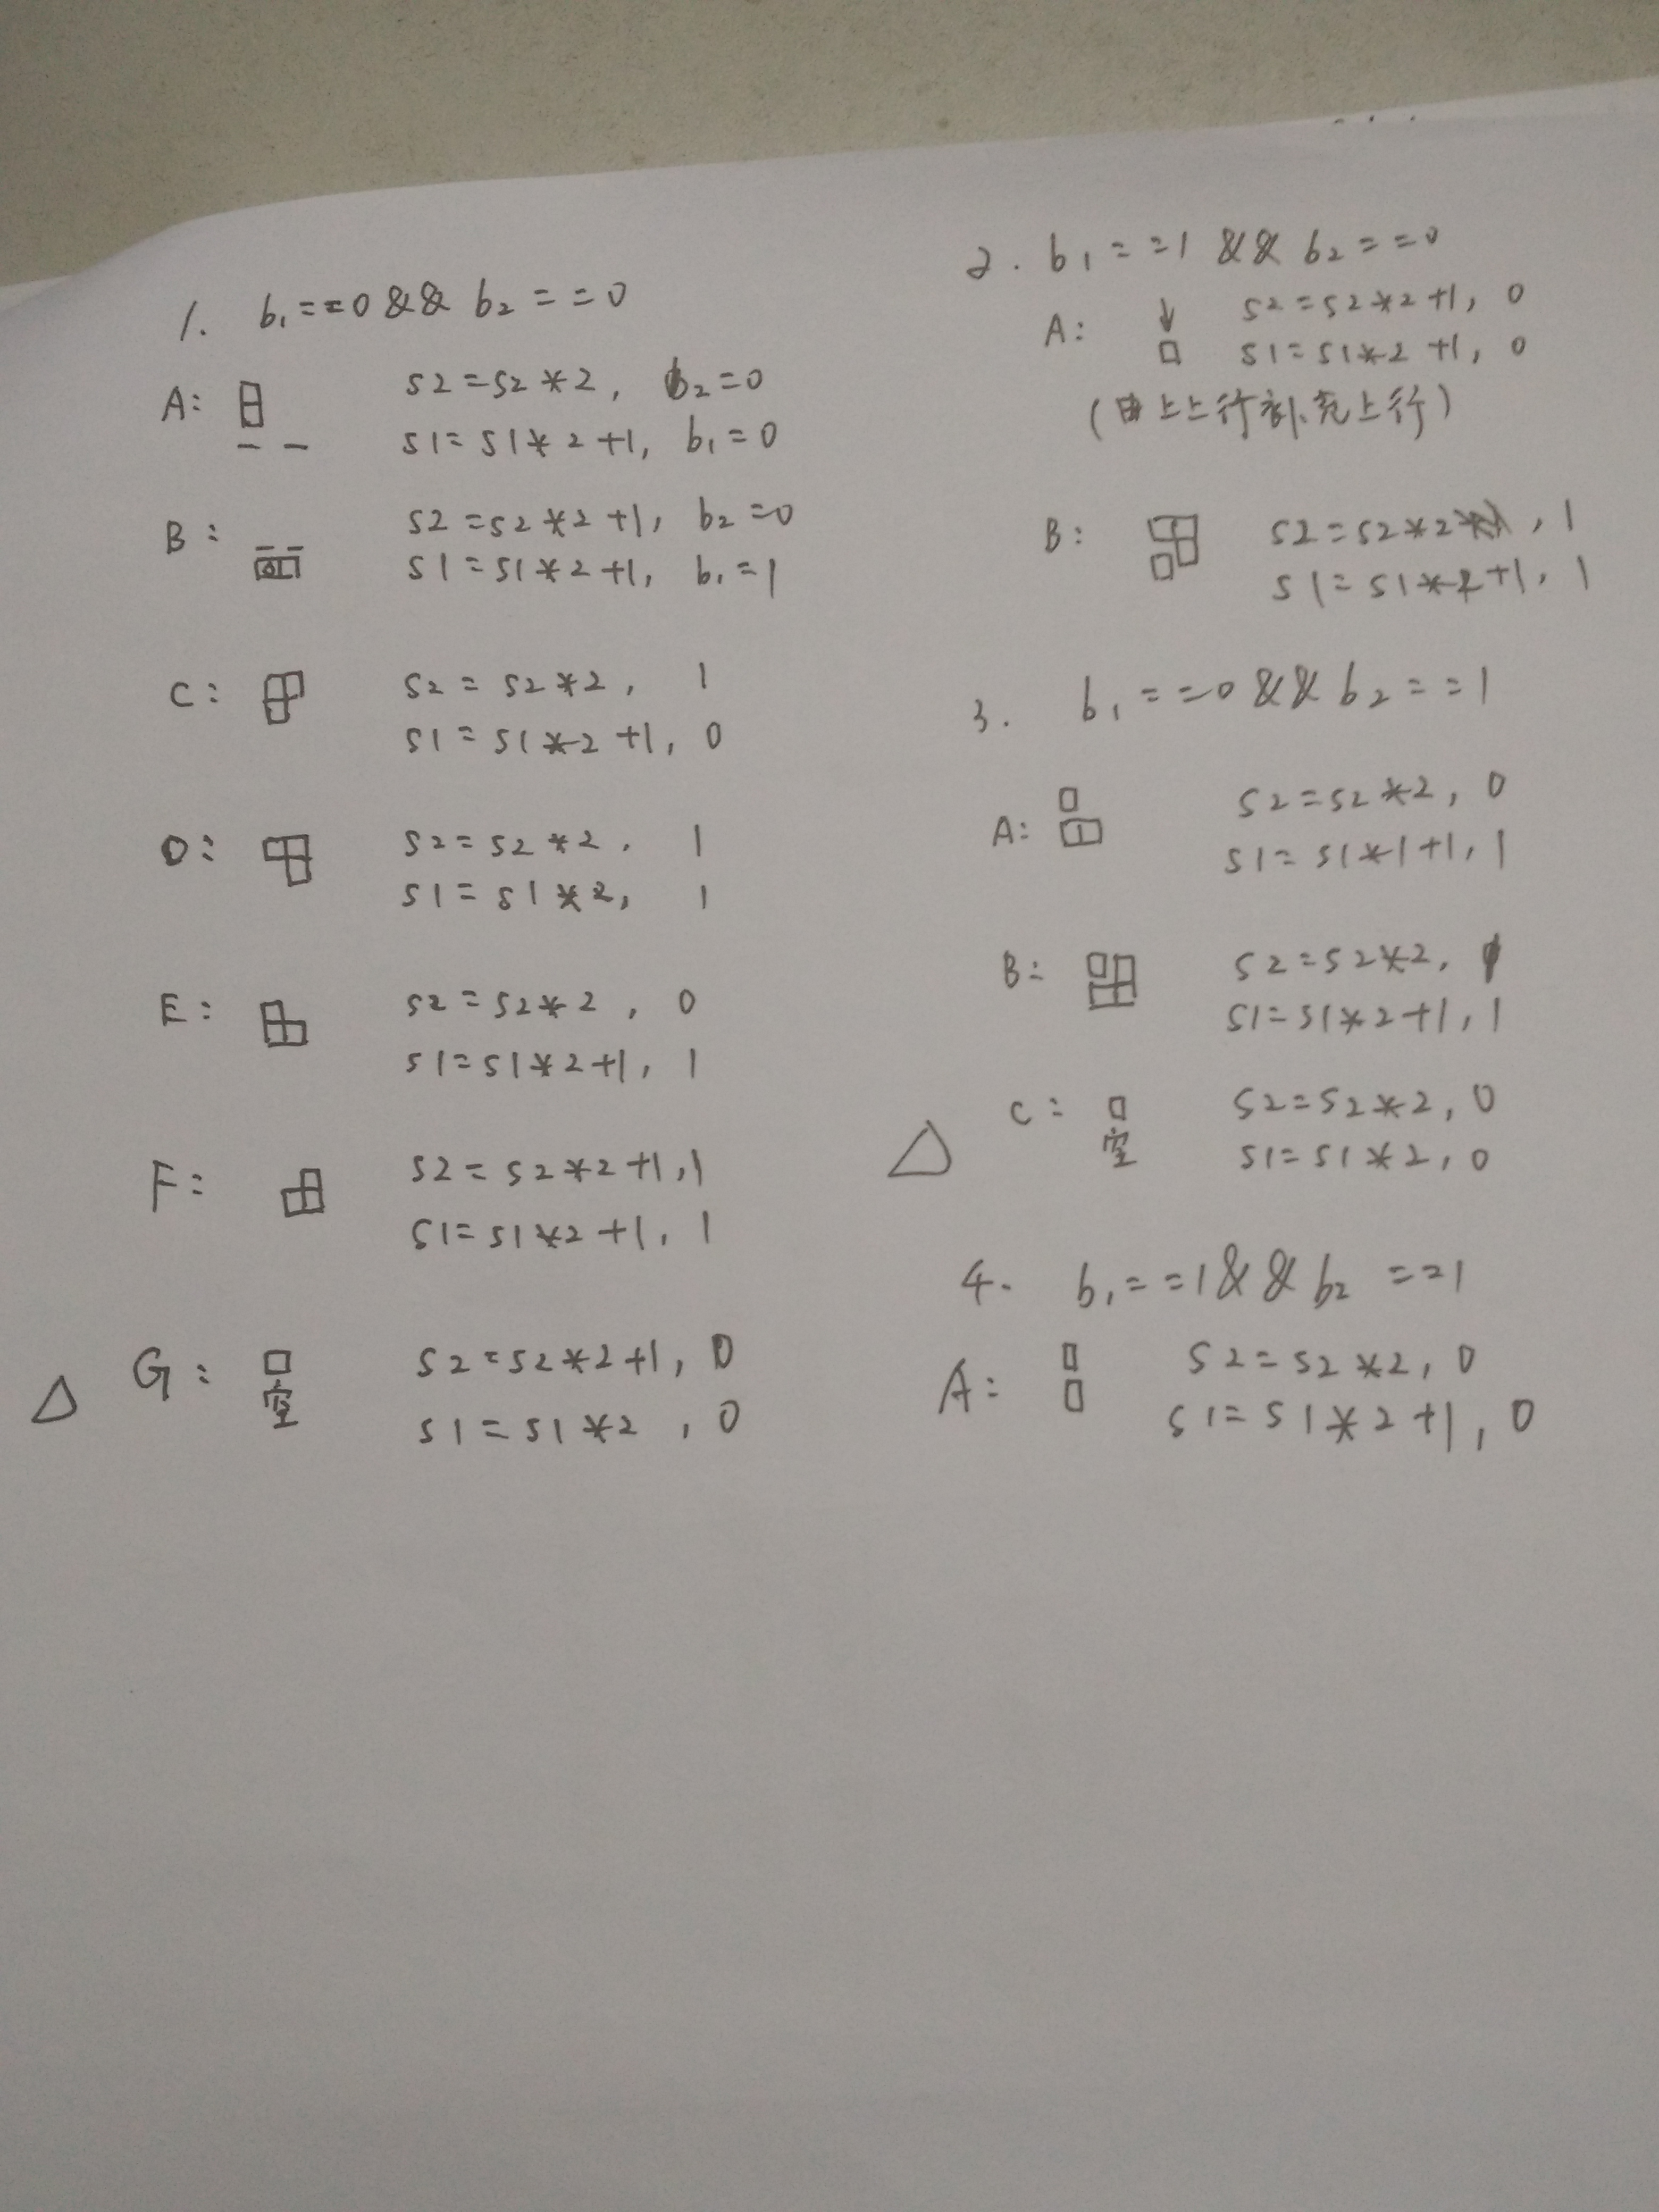
\includegraphics[height = 14cm,width = 17cm]{SCR.jpg}
\begin{lstlisting}
const int MAX_N = 12;

int n, m;
ll ans[MAX_N][MAX_N], dp[MAX_N][1 << MAX_N];

void dfs(int row, int col, int s1, int b1, int s2, int b2)
{
	if (col > m) return;
	if (col == m) {
		if (b1 == 0 && b2 == 0) dp[row][s1] += dp[row - 1][s2];
		return;
	}
	if (b1 == 0 && b2 == 0) {
		dfs(row, col + 1, s1 << 1 | 1, 0, s2 << 1, 0); // 1A
		dfs(row, col + 1, s1 << 1 | 1, 1, s2 << 1 | 1, 0); // 1B
		dfs(row, col + 1, s1 << 1 | 1, 0, s2 << 1, 1); // 1C
		dfs(row, col + 1, s1 << 1 | 1, 1, s2 << 1 | 1, 1); // 1D
		dfs(row, col + 1, s1 << 1 | 1, 1, s2 << 1, 0); // 1E
		dfs(row, col + 1, s1 << 1, 1, s2 << 1, 1); // 1F
		dfs(row, col + 1, s1 << 1, 0, s2 << 1 | 1, 0); // 1G
	} else if (b1 == 1 && b2 == 0) {
		dfs(row, col + 1, s1 << 1 | 1, 0, s2 << 1 | 1, 0); // 2A
		dfs(row, col + 1, s1 << 1 | 1, 1, s2 << 1, 1); // 2B
	} else if (b1 == 0 && b2 == 1) {
		dfs(row, col + 1, s1 << 1 | 1, 1, s2 << 1, 0); // 3A
		dfs(row, col + 1, s1 << 1 | 1, 1, s2 << 1, 1); // 3B
		dfs(row, col + 1, s1 << 1, 0, s2 << 1, 0); // 3C
	} else { // b1 == 1 && b2 == 1
		dfs(row, col + 1, s1 << 1 | 1, 0, s2 << 1, 0); // 4A
	}
}

ll solve()
{
	memset(dp, 0, sizeof (dp));
	dp[0][(1 << m) - 1] = 1;
	for (int i = 1; i <= n + 1; ++i) {
		dfs(i, 0, 0, 0, 0, 0);
	}
	return dp[n][(1 << m) - 1];
}

int main()
{
	memset(ans, -1, sizeof (ans));
	while (~scanf ("%d%d", &n, &m)) {
		if (m > n) swap(n, m);
		if (ans[n][m] != -1) printf("%lld\n", ans[n][m]);
		else {
			ans[n][m] = ans[m][n] = solve();
			printf("%lld\n", ans[n][m]);
		}
	}
	return 0;
}
\end{lstlisting}
\underline {给出$n*m(n,m\leq 10)$的方格棋盘,用$1*r$的长方形骨牌不重叠地覆盖这个棋盘,求覆盖满的方案数。}\\

先考虑$r=3$时的情况。首先,此问题有解当且仅当$m$或$n$能被$3$整除。更一般的结论是:用$1*r$的骨牌覆盖满$m*n$的棋盘,则问题有解当且仅当 $m$或$n$能被$r$整除。当$r=2$时,则对应于例1中$m、n$至少有一个是偶数的条件。 \\
把每一列的状态表示成一个$r$进制数,对于$r=3$,我们用$dp[i][s]$表示把前 $i-2$行覆盖满、第$i-1$和第$i$行覆盖状态为$s$的覆盖方案数。对于第$p$列,$s_p=0$表示$s_{1p}=s_{2p}=0$;$s_{p}=1$表示$s_{1p}=0,s_{2p}=1$;$s_{p} = 2 $表示$s_{1p}=s_{2p}=1$。这样,我们就只保留了必要的状态,空间和时间上都有了改进。当$r= 4$时,可以类推,用四进制表示三行的状态,$r=5$时用五进制……分别写出$r= 2,3,4,5$ 的程序,进行归纳,统一DFS的形式,可以把$DFS(p,s1,s2)$分为两部分:
\begin{lstlisting}
1. for i = 0 to r -1 do
    DFS(p + 1, s1 * r + i, s2 * r + (i + 1) mod r) ;
2. DFS(p + r, s1 * r^r + r^r - 1, s2 * r^r + r^r - 1);
\end{lstlisting}
问题解决。但DFS的这种分部方法是我们归纳猜想得到的,并没有什么道理,其正确性无法保证,我们能否通过某种途径证明它的正确性呢?仍以$r=3$为例。根据上面的讨论,$s_p$取值0到2,表示两行第$p$位的状态,但$s_p$并没有明确的定义。我们**定义$s_p$为这两行的第$p$位从上面一行开始向下连续的1的个数**,这样的定义可以很容易地递推,递推式同上两例没有任何改变,却使得上述DFS方法变得很自然。
\begin{lstlisting}
const int MAX_N = 11;
const int MAX_R = 11;
const int LIMIT = 9800000;

int n, m, r;
ll dp[MAX_N][LIMIT], ans[MAX_N][MAX_N][MAX_R], rr, rm;

void dfs(int row, int col, int s1, int s2)
{
	if (col > m) return;
	if (col == m) {
		dp[row][s1] += dp[row - 1][s2];
		return;
	}
	for (int i = 0; i < r; ++i) {
		dfs(row, col + 1, s1 * r + i, s2 * r + (i + 1) % r);
	}
	dfs(row, col + r, s1 * rr + rr - 1, s2 * rr + rr - 1); // 横着放
}

ll solve()
{
	memset(dp, 0, sizeof (dp));
	rm = rr = 1;
	for (int i = 0; i < r; ++i) { rr *= r; }
	for (int i = 0; i < m; ++i) { rm *= r; }
	dp[0][rm - 1] = 1;
	for (int i = 1; i <= n; ++i) {
		dfs(i, 0, 0, 0);
	}
	return dp[n][rm - 1];
}

int main()
{
	memset(ans, -1, sizeof (ans));
	while (~scanf("%d%d%d", &n, &m, &r)) {
		if (m > n) swap(n, m);
		if (ans[n][m][r] != -1) printf("%lld\n", ans[n][m][r]);
		else if (n * m % r || r > n) printf("0\n");
		else {
			ans[n][m][r] = ans[m][n][r] = solve();
			printf("%lld\n", ans[n][m][r]);
		}
	}
	return 0;
}
\end{lstlisting}

\underline {[PKU 1038]}

给出$m(n\leq 150,m\leq 10)$的棋盘,要在上面放置$2*3$的骨牌,有一些方格无法放置,求最多能放置多少个。\\

根据上例的讨论,此题可以使用三进制来表示状态。$s_p$取值0到2,表示两行第$p$位的状态,**定义$s_p$为这两行的第$p$位从上面一行开始向下连续的1的个数**。我们依旧用$s1$表示当前行状态,$s2$表示上一行状态,$p$表示位置,$num$表示从状态$s1$转移到$s2$能增加的骨牌个数。\\
对于当前行第$p$位,如果放置骨牌,则有两种放置方式:
\begin{enumerate}
\item 竖放,$s1$当前位置$p$及后一个位置$p+1$都为2,s2要求$p$和$p+1$列留空2格,即$p,p+1$列都为0,这样能刚好放置一块骨牌且不留空隙。对应的DFS调用方式:$DFS(p + 2, s1 * 9 + 8, s2 * 9, num + 1)$ ;
\item 横放,$s1$的三个位置都要填满,即$p,p+1,p+2$列均为2,$s2$要求$p,p+1,p+2$列均为1,调用$DFS(p + 3, s1 * 27 + 26, s2 * 27 + 13, num + 1)$
\end{enumerate}
如果第$p$位不放置骨牌,我们还要把$s2$的状态转移到$s1$中以备下次继续转
移。形象地说就是虚填一些方块使得下次放置骨牌可以不留空隙(\underline {也就是填满所有的位置,但是num并不会增加})。对于某一位置,我们可以分3种情况 DFS 以达到目的。
\begin{enumerate}
\item $s1$的当前行空闲,上一行放满。这个状态可以由$s2$的放满状态转移得到:$DFS(p + 1,s1 * 3 + 1, s2 * 3 + 2, num)$
\item $s1$的当前行和上一行都空闲。这个状态可以由$s2$的当前行空闲,上一行放满的状态转移得到:$DFS(p + 1, s1 * 3, s2 * 3 + 1, num)$
\item $s1$的当前行放满。可以由$s2$的放满状态转移得到:$DFS(x + 1, s1 * 3 + 2, s2 * 3 + 2, num)$(放置了1*1的虚骨牌在$s1$的当前位置)
\end{enumerate}
剩下的是关于不能放置的点(黑点)的处理技巧。可以开两个数组$vertical[i][j],horizonal[i][j]$来标志$(i,j)$位置是否能放置竖放和横放骨牌。每次读进一个不能放置的点,对于$vertical[][]$,就把以这个位置为右上角的2*3的六个位置标记掉,对于$horizonal[][]$,就把以这个位置为右上角的3*2的六个位置标记掉,然后在DFS的时候,判断一下就好了。
\begin{lstlisting}
const int MAX_N = 155;
const int MAX_M = 15;
const int MAX_S = 60000;

int T, n, m, K, cur;
int vertical[MAX_N][MAX_M], horizontal[MAX_N][MAX_M];
int dp[MAX_S][2], pw3[MAX_M];

void dfs(int row, int col, int s1, int s2, int num)
{
	if (col > m) return;
	if (col == m) {
		dp[s1][cur] = max(dp[s1][cur], dp[s2][cur ^ 1] + num);
		return;
	}
	if (row >= 2 && vertical[row][col] == 0) { // 竖放
		dfs(row, col + 2, s1 * 9 + 8, s2 * 9, num + 1);
	}
	if (row >= 1 && horizontal[row][col] == 0) { // 横放
		dfs(row, col + 3, s1 * 27 + 26, s2 * 27 + 13, num + 1);
	}
	dfs(row, col + 1, s1 * 3, s2 * 3 + 1, num);
	dfs(row, col + 1, s1 * 3 + 1, s2 * 3 + 2, num);
	dfs(row, col + 1, s1 * 3 + 2, s2 * 3 + 2, num);
}

void solve()
{
	memset(dp, 0, sizeof (dp));
	cur = 0;
	for (int i = 1; i < n; ++i) {
		cur ^= 1;
		dfs(i, 0, 0, 0, 0);
	}
	int ret = 0;
	for (int i = 0; i < pw3[m]; ++i) {
		ret = max(ret, max(dp[i][cur], dp[i][cur ^ 1]));
	}
	printf("%d\n", ret);
}

int main()
{
	pw3[0] = 1;
	for (int i = 1; i < 12; ++i) { pw3[i] = 3 * pw3[i - 1]; }
	scanf("%d", &T);
	while (T--) {
		scanf("%d%d%d", &n, &m, &K);
		memset(vertical, 0, sizeof (vertical));
		memset(horizontal, 0, sizeof (horizontal));
		for (int i = 0; i < K; ++i) {
			int x, y;
			scanf("%d%d", &x, &y);
			x--, y--;
			vertical[x][y] = vertical[x + 1][y] = vertical[x + 2][y] = 1;
			if (y > 0) vertical[x][y - 1] = vertical[x + 1][y - 1]
                                        = vertical[x + 2][y - 1] = 1;
			horizontal[x][y] = horizontal[x + 1][y] = 1;
			if (y > 0) horizontal[x][y - 1] = horizontal[x + 1][y - 1] = 1;
			if (y > 1) horizontal[x][y - 2] = horizontal[x + 1][y - 2] = 1;
		}
		solve();
	}
	return 0;
}
\end{lstlisting}

\subsection{图论模型}
\underline {[HDU 4917]}

给一个$n(n\leq 40)$个顶点和$m(m\leq 20)$个已知拓扑关系的图,求这个图合法的拓扑排序的个数。\\

已知的$m$个拓扑关系会将图分成若干个联通块,但是每个联通块的内部顶点数量不会超过20(因为$m\leq 20$)。我们把一个含有$num$个顶点的连通块内部可以形成的合法拓扑排序的方案数记为$SCR(num)$,当前还剩下$left$个顶点没被确定(包括连通块内的$num$个顶点)那么此时可得的方案数是:$SCR(num)*C[left][num]$,这个组合数的含义其实就是把这$num$个顶点按顺序放在$left$个顶点的任意$num$个位置都是可以的,根据乘法原理,每个连通块的答案要相乘,同时$left$要减掉$num$。 \\
那么剩下来两个问题,如何确定每个连通块内部的顶点和求$SCR(num)$?对于第一个问题,我们可以建立一个0/1邻接矩阵:$child[u][v]$,当$child[u][v]=1$时表示$u$有一个儿子$v$(根据读进来的$m$个关系确定),否则$child[u][v]=0$,对于每个连通块内部点我们可以借鉴\underline {最短路中Floyd算法}的思路,$n^3$的复杂度把这个邻接矩阵“补全”,也就是所有点的所有儿子都标记得到。同一连通块可以通过\underline {并查集}判断得到。同时要把所有的同一连通块中的顶点重新编号。 \\
对于第二个问题,我们同样枚举状态$s: 1\rightarrow ((1 << s) -1)$,把$s$二进制表示中的1看成已经排好序的点,只需要枚举最后一个点是谁,但是要满足\underline {这个点的所有父亲都已经排好序了},把$v$的父亲节点信息同样用一个二进制数$pre[v]$保存就好了,只要状态$s\& pre[v]=pre[v]$,那么就说明状态$s$中包含了所有$v$的父亲。这里是\underline {集合的思想}。 \\
时间复杂度是比较高的:$O(n*2^{num}*num)$,时限给了1000ms,下面的代码跑了795ms。

\begin{lstlisting}
const ll mod = (ll)(1e9 + 7);

int n, m;
int child[45][45], vis[45], fa[45], id[45], step[45], pre[45];
ll dp[1 << 21], C[45][45];

void Floyd()
{
	for (int i = 1; i <= n; ++i) {
		for (int j = 1; j <= n; ++j) {
			if (child[i][j] == 0) continue;
			for (int k = 1; k <= n; ++k) {
				if (child[j][k] == 0) continue;
				child[i][k] = 1;
			}
		}
	}
}

int find(int x)
{
	return fa[x] == x ? x : fa[x] = find(fa[x]);
}

int GetConnectedGraph(int st)
{
	int ret = 0, ancestor = find(st);
	memset(pre, 0, sizeof (pre));
	for (int i = st; i <= n; ++i) {
		if (vis[i]) continue;
		int fi = find(i);
		if (fi == ancestor) {
			id[ret] = i;
			step[i] = ret++;
			vis[i] = 1;
		}
	}
	for (int i = 0; i < ret; ++i) {
		int v = id[i];
		for (int u = 1; u <= n; ++u) {
			if (child[u][v]) {
				pre[v] += (1 << step[u]);
			}
		}
	}
	return ret;
}	

ll SCR(int num)
{
	memset(dp, 0, sizeof (dp));
	dp[0] = 1;
	for (int s = 1; s < (1 << num); ++s) {
		for (int i = 0; i < num; ++i) {
			if ((1 << i) > s) break;
			if ((1 << i) & s) {
				int v = id[i], ss = s - (1 << i);
				int tmp = (pre[v] & ss);
				if (tmp == pre[v]) {
					dp[s] += dp[ss];
					if (dp[s] >= mod) dp[s] -= mod;
				}
			}
		}
	}
	return dp[(1 << num) - 1];
}

ll solve()
{
	Floyd();
	memset(vis, 0, sizeof (vis));
	ll ret = 1;
	int left = n;
	for (int i = 1; i <= n; ++i) {
		if (vis[i]) continue;
		int num = GetConnectedGraph(i);
		ll tmp = SCR(num);
		ret = ret * C[left][num] % mod * tmp % mod;
		left -= num;
	}
	return ret;
}

int main()
{
	for (int i = 0; i < 45; ++i) {
		C[i][0] = C[i][i] = 1;
		for (int j = 1; j < i; ++j) {
			C[i][j] = C[i - 1][j] + C[i - 1][j - 1];
			if (C[i][j] >= mod) C[i][j] -= mod;
		}
	}
	while (~scanf ("%d%d", &n, &m)) {
		memset(child, 0, sizeof (child));
		for (int i = 0; i <= n; ++i) { fa[i] = i; }
		for (int i = 0; i < m; ++i) {
			int u, v, fu, fv;
			scanf("%d%d", &u, &v);
			child[u][v] = 1;
			fu = find(u), fv = find(v);
			if (fu != fv) { fa[fv] = fu; }
		}
		printf("%lld\n", solve());
	}
	return 0;
}
\end{lstlisting}
通过一种DFS的方式获得每个连通块内部的点,并打标记,效果比较好,只跑了592ms。 \\
同样是邻接矩阵$link[i][j]$:
\begin{itemize}
\item $link[i][j]=1:i$是$j$的父亲
\item $link[i][j]=-1:j$是$i$的父亲
\item $link[i][j]=0:i$和$j$不存在直接系
\end{itemize}

\begin{lstlisting}
void dfs(int u, int& num)
{
	id[num] = u;
	vis[u] = 1;
	int tmp = num++; // 暂时保存 u 的编号顺序
	for (int i = 1; i <= n; ++i) {
		if (link[u][i] != 0) { // 父亲方向,儿子方向都遍历
			if (!vis[i]) dfs(i, num); // 遍历 i 的所有儿子和父亲
			if (link[u][i] == 1) { // 遍历 u 的所有儿子
				for (int j = 0; j < num; ++j) {
					if (id[j] == i) { // 找到 i
						pre[j] |= (1 << tmp);
						break;
					}
				}
			}
		}
	}
`}
\end{lstlisting}

\underline {[BZOJ 2784]}

求$n(n\leq 10^5)$以内所有数构成的满足下列条件的集合的个数:如果$x$在这个集合内,那么$2x,3x$都不能在这个集合内。例如:$n=4$,符合条件的子集是:$\{1\},\{1,4\},\{2\},\{2,3\},\{3\},\{3,4\},\{4\}$,一共8个。

需(hen)要(nan)想到这样一个数字矩阵: \\ \\
\begin{tabular}{|c|c|c|c|c|}%开始绘制表格
%{|c|c|c|c|c|} 表示会有5列, 每个的方式未居中(c),
%也可以改成靠左(l)和靠右(r) 其中 | 表示绘制列线
\hline %绘制一条水平的线
x  &  3x &  9x  & 27x  & \dots \\
\hline
2x &  6x & 18x  & 54x  & \dots \\
\hline
4x & 12x & 36x  & 108x & \dots \\
\hline
\dots & \dots & \dots & \dots & \dots \\
\hline
\end{tabular}

这样的数字矩阵最多会有:17行11列。对于每行的数字显然不能取左右相邻的,对于相邻行的状态显然不能同一列都取。每种矩阵方案先构造矩阵,然后状压dp+滚动数组递推,对于所有的可能矩阵方案乘法原理连乘即可。 \\
虽然时限给了10s,但是实际上AC只要660MS。

\begin{lstlisting}
int n;
int mat[18][13], vis[MAX_N], col[18];
ll dp[2][1 << 12];

ll wyr(int x)
{
	int row;
	// 构造矩阵
	for (int i = 1; ; ++i) {
		if (i == 1) mat[i][0] = x;
		else mat[i][0] = 2 * mat[i - 1][0];
		if (mat[i][0] > n) {
			row = i - 1;
			break;
		}
		vis[mat[i][0]] = 1;
		for (int j = 1; ; ++j) {
			mat[i][j] = mat[i][j - 1] * 3;
			if (mat[i][j] > n) {
				col[i] = j; // 每一行的列数
				break;
			}
			vis[mat[i][j]] = 1;
		}
	}
	memset(dp, 0, sizeof (dp));
	dp[0][0] = 1, col[0] = 0;
	int cur = 0;
	ll ret = 0;
	for (int i = 1; i <= row; ++i) {
		cur ^= 1;
		memset(dp[cur], 0, sizeof (dp[cur]));
		for (int s = 0; s < (1 << col[i]); ++s) {
			if (s & (s << 1)) continue; // 同一行不能取相邻
			for (int pre = 0; pre < (1 << col[i - 1]); ++pre) {
				if (dp[cur ^ 1][pre] == 0 || (pre & s)) continue;
				// 上一行状态存在并且不能取相邻列
				dp[cur][s] += dp[cur ^ 1][pre];
				if (dp[cur][s] >= mod) dp[cur][s] -= mod;
			}
			if (i == row) {
				ret += dp[cur][s];
				if (ret >= mod) ret -= mod;
			}
		}
	}
	return ret;
}

int main()
{
	scanf("%d", &n);
	ll ans = 1;
	for (int i = 1; i <= n; ++i) {
		if (vis[i] == 0) {
			ans = ans * wyr(i) % mod;
		}
	}
	printf("%lld\n", ans);
	return 0;
}
\end{lstlisting}

\clearpage
\section{dp优化}

\subsection{二进制优化}
\underline{[HDU 1171]} \\

$n\leq 1000$件商品,每件商品的数量和单价为$num[i]\leq 100$和$value[i]$,求将这些商品尽可能分成价值相等的两部分,输出两部分价值$A$和$B$($A\geq B$)。 \\

把每种商品的数量二级制拆分成“另一种”商品。 \\
将一部分$O(\sum (num[i]))$的时间复杂度降为:$O(\sum{\log (num[i])})$
\begin{lstlisting}
const int MAX_N = 1010;

int sum, n, total;
int value[MAX_N], num[MAX_N], good[MAX_N * 15], dp[100010];

int main()
{
	while (~scanf("%d", &n) && n >= 0) {
		sum = total = 0;
		for (int i = 0; i < n; ++i) {
			scanf("%d%d", &value[i], &num[i]);
			sum += value[i] * num[i];
			for (int j = 1; j <= num[i]; j <<= 1) {
				good[total++] = j * value[i];
				num[i] -= j;
			}
			if (num[i]) good[total++] = num[i] * value[i];
		}
		memset(dp, 0, sizeof (dp));
		dp[0] = 1;
		int half = sum / 2;
		for (int i = 0; i < total; ++i) {
			for (int j = half; j >= good[i]; --j) {
				if (dp[j - good[i]]) {
					dp[j] = 1;
				}
			}
		}
		for (int i = half; i >= 0; --i) {
			if (dp[i]) {
				printf("%d %d\n", sum - i, i);
				break;
			}
		}
	}
	return 0;
}
\end{lstlisting}

\subsection{单调队列优化}
\underline{[POJ 3401]} \\

已知$n\leq 2000$天每天买卖一张股票的单价和买卖上限,但是每天只能选择买或者卖或者不交易,而且两次交易日期中间至少要间隔$W$ 天,最多可以持有$Max$张股票。初始时有无限量的钱,求最终最多可以获利多少? \\

用$dp[i][j]$表示在第$i$天拥有$j$张股票时的最多获利。
\begin{itemize}
\item 第$i$天不买不卖:$dp[i][j]=dp[i - 1][j]$
\item 第$i$天买股票:$dp[i][j]=max(dp[r][k]-cost[i]*(j-k))\quad (r\leq i - W - 1,k< j)$
\item 第$i$天卖股票:$dp[i][j]=max(dp[r][k]+value[i]*(k-j))\quad (r\leq i - W - 1,k> j)$
\end{itemize}
考虑实际意义上面式子中的$r$就应该是$i-W-1$。把第二种情况的状态转移改写一下:
$$
dp[i][j]=(dp[i-W-1][k]+buy[i]*k)-buy[i]*j \qquad (k< j)
$$
可以发现前面部分就是求前缀最大,所以可以用单调队列来保存前缀最大。对于卖股票的行为同样处理,但是因为$k>j$,所以要倒着处理。
\begin{lstlisting}
const int MAX_N = 2010;
const int inf = 0x3f3f3f3f;

int T, n, Max, W, head, tail;
int cost[MAX_N], value[MAX_N], buy[MAX_N], sell[MAX_N];
// cost 和 value: 买卖单价, buy 和 sell: 买卖上限
int dp[MAX_N][MAX_N];

struct Que {
	int num, sum;
	// num: 股票数量 sum: 已经获利量
	Que() {}
	Que(int _num, int _sum): num(_num), sum(_sum) {}
} que[MAX_N];

void wyr()
{
	for (int i = 0; i < n; ++i) memset(dp[i], -0x3f, sizeof (dp[i]));
	// 预处理前 W 天
	for (int j = 0; j <= buy[0]; ++j) { dp[0][j] = -j * cost[0]; }
	for (int i = 1; i <= W; ++i) {
		for (int j = 0; j <= Max; ++j) {
			dp[i][j] = dp[i - 1][j];
			if (j <= buy[i]) dp[i][j] = max(dp[i][j], -j * cost[i]);
		}
	}
	for (int i = W + 1; i < n; ++i) {
		head = tail = 0;
		for (int j = 0; j <= Max; ++j) {
			dp[i][j] = dp[i - 1][j]; // 不买不卖
			
			// 买
			while (head < tail && que[tail - 1].sum <
                                dp[i - W - 1][j] + j * cost[i]) {
				tail--;
			}
			que[tail++] = Que(j, dp[i - W - 1][j] + j * cost[i]);
			// 保证买的数量不超过上限
			while (head < tail && j - que[head].num > buy[i]) head++;
			dp[i][j] = max(dp[i][j], que[head].sum - j * cost[i]);
		}

		head = tail = 0; // 卖
		for (int j = Max; j >= 0; --j) {
			while (head < tail && que[tail - 1].sum <
                            dp[i - W - 1][j] + j * value[i]) {
				tail--;
			}
			que[tail++] = Que(j, dp[i - W - 1][j] + j * value[i]);
			while (head < tail && que[head].num - j > sell[i]) head++;
			dp[i][j] = max(dp[i][j], que[head].sum - j * value[i]);
		}
	}
	int ans = 0;
	for (int i = 0; i <= Max; ++i) {
		ans = max(ans, dp[n - 1][i]);
	}
	printf("%d\n", ans);
}

int main()
{
	scanf("%d", &T);
	while (T--) {
		scanf("%d%d%d", &n, &Max, &W);
		for (int i = 0; i < n; ++i) {
			scanf("%d%d%d%d", &cost[i], &value[i], &buy[i], &sell[i]);
		}
		wyr();
	}
	return 0;
}
\end{lstlisting}

\underline {POJ 3245}

一个长度为$n\leq 5*10^4$的序列(每个元素是($a_i,b_i$)这样的数对),连续地分成若干组。每组左右边界是($l_1,r_1$),($l_2,r_2$),$\cdots$,($l_p,r_p$),满足$l_i=r_{i−1}+1,l_i
\leq r_i,l_1=1,r_p=n$。分组必须满足两个条件:前面组的元素的$b$值比后面组元素的所有$a$值大;令$M_i$为第$i$个组内最大的$a$,所有$M_i$的和不超过$limit$。令$S_i$为第$i$个组的元素的$b$的和,最小化$max\{S_i\}$。 \\

只要有数列后面的$a_j$大于等于当前的$b_i$,那么$i$到$j$的所有元素必须在一个块,那么就把他们合并,合并就是$a$取最大值,$b$取和。此时问题就变成了把这些点分成若干组,且各个组的$M_i$之和要满足限制条件,求$max\{S_i\}$最小是多少,$S_i$表示第$i$组中各个点的$b$值之和。二分$max\{S_i\}$的最小值$x$,然后将问题转变成:将这些点分成若干组,且每组的$b$值之和不能超过$x$,求各个组的$M_i$之和也就各个组的$a$的最大值之和最小是多少,并且判断一下是否小于或等于$limit$。 \\
状态转移方程:
$$
dp[i] = max(dp[j] + max(a[j+1], a[j+2], ..., a[i])) \quad sum[i]-sum[j]\leq M
$$
决策点具有单调性:在决策区间内维护一个单调下降的序列,缩小决策点的数目。需要使用multiset。

时间复杂度:$O(n\log n)$
\begin{lstlisting}
const int MAX_N = 50010;
const int inf = 0x3f3f3f3f;

int n, limit, head, tail;
int A[MAX_N], B[MAX_N], newA[MAX_N], newB[MAX_N], flag[MAX_N];
int pre[MAX_N], suf[MAX_N], sum[MAX_N], dp[MAX_N], Q[MAX_N];
multiset<int> mst;

int check(int x)
{
	dp[0] = Q[0] = head = 0, tail = -1;	
	int st = 1;
	mst.clear();
	for (int i = 1; i <= n; ++i) {
		if (newB[i] > x) return 0;
		while (sum[i] - sum[st - 1] > x) st++; // st 是区间左端点,闭区间
		while (head <= tail && newA[i] >= newA[Q[tail]]) { // 维护队列单调递减性
			if (head < tail) mst.erase(dp[Q[tail - 1]] + newA[Q[tail]]); // 剔除值
			--tail;
		}
		Q[++tail] = i;
		if (head < tail) mst.insert(dp[Q[tail - 1]] + newA[i]); // 增加值
		while (Q[head] < st) { // 将队列首元素位置调到区间内
			if (head < tail) mst.erase(dp[Q[head]] + newA[Q[head + 1]]); // 剔除值
			++head;
		}
		dp[i] = dp[st - 1] + newA[Q[head]]; // 获得 dp 值
		if (head < tail && dp[i] > (*mst.begin())) dp[i] = *mst.begin();
		// mst 中所有值都是 dp[i] 的候选项
		if (dp[i] > limit) return 0;
	}
	return 1;
}

void merge()
{
	suf[n + 1] = 0, pre[0] = INT_MAX;
	for (int i = 1; i <= n; ++i) {
		pre[i] = min(pre[i - 1], B[i]);
	}
	for (int i = n; i >= 1; --i) {
		suf[i] = max(suf[i + 1], A[i]);
	}
	memset(newA, 0, sizeof (newA));
	memset(newB, 0, sizeof (newB));
	memset(flag, 0, sizeof (flag));
	for (int i = 1; i <= n; ++i) {
		if (pre[i] > suf[i + 1]) flag[i] = 1;
	}
	int total = 1;
	for (int i = 1; i <= n; ++i) {
		newA[total] = max(newA[total], A[i]);
		newB[total] += B[i];
		if (flag[i]) total++;
	}
	n = total - 1;
	sum[0] = 0;
	for (int i = 1; i <= n; ++i) {
		sum[i] = sum[i - 1] + newB[i];
	}
}

void solve()
{
	merge();
	int low = 1, high = sum[n], mid;
	while (low < high) {
		mid = (low + high) >> 1;
		if (check(mid)) high = mid;
		else low = mid + 1;
	}
	printf("%d\n", high);
}

int main()
{
	while (~scanf("%d%d", &n, &limit)) {
		for (int i = 1; i <= n; ++i) {
			scanf("%d%d", &A[i], &B[i]);
		}
		solve();
	}
	return 0;
}
\end{lstlisting}

\subsection{斜率优化}
\underline {[POJ 1180]} \\

有$n\leq 10^4$件商品需要加工,每件商品有两个属性:$O(i)$和$F(i)$,可以把连续的一些商品看成一组一起加工,每加工一组需要$S$ 的时间起动机器,假设在时刻$t$开始加工从$i\sim j$的商品,那么加工完这些商品的耗时是:$t+S+\sum_{r=i}^{r=j}{O(r)}=t+T$,需要的代价是:$(t+T)*\sum_{r=i}^{r=j}{F(r)}$,并且下一组的开始时刻是$t+T$,初始时刻是0。求加工完这些商品的最小代价? \\

可以发现每加工完一组商品的这部分时间:$T=S+\sum_{r=i}^{r=j}{O(r)}$对于后面的所有商品都是有影响的,可以先把这部分影响计算累加,影响是:
$$T*\sum_{r=i+1}^{n}{F(r)}=T*fsum(j)$$
于是用$dp[i]$表示加工完$i\sim n$商品的最小代价,$tsum[i]$和$fsum[i]$表示分别$O[]$和$F[]$的后缀和。
$$
dp[i]=min(dp[j]+(S+tsum[i]-tsum[j])*fsum[i])\quad (i< j\leq n)
$$
斜率方程:
$$
\frac{dp[x]-dp[y]}{tsum[x]-tsum[y]}\leq fsum[i]
$$

\begin{lstlisting}
ll G(int x, int y)
{
	return dp[x] - dp[y];
}

ll S(int x, int y)
{
	return tsum[x] - tsum[y];
}

void solve()
{
	head = tail = 0;
	Q[0] = n + 1;
	dp[n + 1] = 0;
	for (int i = n; i >= 1; --i) {
		while (head < tail && G(Q[head + 1], Q[head]) <=
				fsum[i] * S(Q[head + 1], Q[head])) ++head;
		dp[i] = dp[Q[head]] + (tsum[i] - tsum[Q[head]] + s) * fsum[i];
		while (head < tail && G(Q[tail], Q[tail - 1]) * S(i, Q[tail]) >
				G(i, Q[tail]) * S(Q[tail], Q[tail - 1])) --tail;
		Q[++tail] = i;
	}
	printf("%lld\n", dp[1]);
}
\end{lstlisting}

\underline {[HDU 3669]} \\

给出$n\leq 5*10^4$个矩形的长和宽,要求把这些矩形最多分成$K$组,每组的代价是所有这组矩形的最大宽乘以最大长。求最小代价和?\\

先把矩形按照优先宽度:从大到小,其次高度:从大到小的顺序排序,其次要注意到一个事实:如果一个矩形的宽和长都比另外一个矩形小,那个这个矩形就是不用考虑的。因此我们根据排序后的矩形筛选出的矩形序列满足这样性质:宽递减并且长递增。 \\
用$dp[i][k]$表示将前$i$个矩形分成$k$组的最小代价:
$$
dp[i][k]=min(dp[j][k-1]+rec[j+1].w*rec[i].h) \quad (j< i)
$$
斜率方程:
$$
\frac{dp[x][p-1]-dp[y][p-1]}{rec[y+1].w-rec[x+1].w}\leq rec[i].h
$$
\begin{lstlisting}
int n, K, head, tail;
int Q[MAX_N];
ll dp[MAX_N][MAX_K];

struct Rec {
	int w, h;
	bool operator < (const Rec& rhs) const {
		if (w != rhs.w) return w > rhs.w;
		else return h > rhs.h;
	}
} read[MAX_N], rec[MAX_N];

ll G(int id, int x, int y)
{
	return dp[x][id] - dp[y][id];
}

ll S(int x, int y)
{
	return rec[y + 1].w - rec[x + 1].w;
}

void wyr()
{
	for (int i = 1; i <= n; ++i) {
		dp[i][1] = 1ll * rec[1].w * rec[i].h;
	}
	for (int k = 2; k <= K; ++k) {
		head = tail = 0;
		Q[++tail] = k - 1;
		for (int i = k; i <= n; ++i) {
			while (head < tail && G(k - 1, Q[head + 1], Q[head])
					<= S(Q[head + 1], Q[head]) * rec[i].h) ++head;
			int t = Q[head];
			dp[i][k] = dp[t][k - 1] + 1ll * rec[t + 1].w * rec[i].h;
			while (head < tail && G(k - 1, Q[tail], Q[tail - 1]) * S(i, Q[tail])
					>= G(k - 1, i, Q[tail]) * S(Q[tail], Q[tail - 1])) --tail;
			Q[++tail] = i;
		}
	}
	ll ans = (ll)(1e18);
	for (int i = 1; i <= K; ++i) {
		ans = min(ans, dp[n][i]);
	}
	printf("%lld\n", ans);
}

int main()
{
	while (~scanf("%d%d", &n, &K)) {
		for (int i = 0; i < n; ++i) {
			scanf("%d%d", &read[i].w, &read[i].h);
		}
		sort(read, read + n);
		int MaxH = 0, total = 0;
		for (int i = 0; i < n; ++i) {
			if (read[i].h > MaxH) {
				rec[++total].w = read[i].w;
				rec[total].h = read[i].h;
				MaxH = read[i].h;
			}
		}
		n = total;
		wyr();
	}
	return 0;
}
\end{lstlisting}

\subsection{四边形不等式优化}
假如对于$i < j$,有:
$$w(i,j)+w(i+1,j+1)\leq w(i+1,j)+w(i,j+1)$$
称函数$w$满足四边形不等式。 \\
将不等式变形得:
$$
w(i+1,j+1)- w(i+1,j)\leq w(i,j+1) - w(i,j)
$$
那么证明函数$w$是否满足四边形不等式,即证明:当$j$固定不变时是否有:$w(i,j+1)-w(i,j)$随$i$非递增。 \\

\begin{itemize}
\item 定理1 \\
如果有状态转移方程:
$$
m(i,j)=\min_{i < k\leq j}\{ m(i,k-1)+m(k,j)+w(i,j)\} \quad (i < j,m(i,i)=0)
$$
那么函数$m$也满足四边形不等式:
$$
m(i,j)+m(i+1,j+1)\leq m(i+1,j)+m(i,j+1),\quad i < j
$$
\item 定理2 \\
定义$s(i,j)$为函数$m(i,j)$对应的决策变量的最大值,即:
$$
s(i,j)=\max_{i < k\leq j}\{m(i,j)=w(i,j)+m(i,k-1)+m(k,j)\}
$$
并且$m(i,j)$满足四边形不等式,那么$s(i,j)$单调,即:
$$
s(i,j)\leq s(i,j+1)\leq s(i+1,j+1)
$$
因此$m(i,j)$的状态转移方程等价于:
$$
m(i,j)=\min_{s(i,j-1) < k \leq s(i+1,j)}\{ m(i,k-1)+m(k,j)+w(i,j)\} \quad (i < j,m(i,i)=0)
$$
这个转移的复杂度是:$O(n^2)$。
\end{itemize}

\underline {环形石子堆合并} \\

[HDU 3506]:给$n\leq 1000$个围成一圈的石子堆,每次可以合并相邻的两个石子堆成一个新的石子堆,合并的代价是两堆石子数量之和,求将$n$堆石子合并成一堆的最小代价? \\

先将$n$堆环形石子展开成一排$2*n$堆石子。用$dp[i][j]$表示合并第$i$堆到第$j$堆石子的最小代价,状态转移方程:
$$
dp[i][j]=min(dp[i][k]+dp[k+1][j])+cost[i][j]\quad (i\leq k\leq j)
$$
利用四边形不等式优化,只需证明:当$j$固定不变时是否有$cost[i][j+1]-cost[i][j]$随$i$单调非递增。
$$
cost[i][j]=\sum_{r=i}^{r=j}data[r] \\
cost[i][j+1]-cost[i][j]=data[j+1]
$$
因为$j$固定不变,所以差值是个恒定值,那么满足随$i$单调非递增(不变)。 \\
时间复杂度:$O(n^2)$
\begin{lstlisting}
const int MAX_N = 1010 * 2;

int n;
int d[MAX_N], sum[MAX_N];
int dp[MAX_N][MAX_N], s[MAX_N][MAX_N];

void solve()
{
	for (int i = 1; i <= 2 * n; ++i) {
		sum[i] = sum[i - 1] + d[i];
	}
	d[2 * n + 1] = d[1];
	for (int i = 1; i < 2 * n; ++i) {
		dp[i][i + 1] = d[i] + d[i + 1];
		s[i][i + 1] = i;
	}
	for (int len = 3; len <= n; ++len) {
		for (int i = 1; i + len - 1 <= 2 * n; ++i) {
			int j = i + len - 1;
			dp[i][j] = INT_MAX;
			int a = s[i][j - 1], b = s[i + 1][j];
			for (int r = a; r <= b; ++r) {
				int tmp = dp[i][r] + dp[r + 1][j] + sum[j] - sum[i - 1];
				if (tmp < dp[i][j]) {
					dp[i][j] = tmp;
					s[i][j] = r;
				}
			}
		}
	}
	int ans = INT_MAX;
	for (int i = 1; i <= n; ++i) {
		ans = min(ans, dp[i][i + n - 1]);
	}
	printf("%d\n", ans);
}

int main()
{
	while (~scanf("%d", &n)) {
		for (int i = 1; i <= n; ++i) {
			scanf("%d", &d[i]);
			d[i + n] = d[i];
			dp[i][i] = 0;
			s[i][i] = i;
		}
		solve();
	}
	return 0;
}
\end{lstlisting}
\underline {[HDU 2829]}

给$n\leq 1000$个正整数,定义下标$i\sim j$的一串连续的没被挡板隔开的数的价值为:$\sum_{p=i}^{p=j}data[p]\sum_{q=p+1}^{q=j}{data[q]}$,只有一个数时价值为0,选择合适的位置放置$K\in [0,n)$个挡板,使得最终的总价值最小,输出最小总价值。 \\

定义:$sum[i]=\sum_{r=1}^{r=i}{data[r]}$,$fsum[i]=\sum_{r=1}^{r=i}data[r]*sum[r]$
$$
\begin{aligned}
cos[i][j]&=\sum_{p=i}^{p=j}data[p]\sum_{q=p+1}^{q=j}{data[q]} \\
&=\sum_{p=i}^{p=j}data[p]*(sum[j]-sum[p]) \\
&=sum[j]*(sum[j]-sum[i-1])-(fsum[j]-fsum[i-1])
\end{aligned}
$$
定义$dp[i][k]$表示在前$i$个数放置$k$个挡板可获得价值,状态转移方程:
$$
dp[i][k]=\min_{0\leq j < i}\{dp[j][k-1]+cost[j+1][i]\}
$$
考虑四边形不等式优化,只需要证明:当$j$固定时,$cost[i][j+1]-cost[i][j]$随$i$单调非增。
$$
\begin{aligned}
cost[i][j+1]-cost[i][j]&=({sum[j+1]}^{2}-fsum[j+1])-({sum[j]}^{2}-fsum[j]) \\
&+(sum[j]-sum[j+1])*sum[i-1]
\end{aligned}
$$
因为$sum[r]$是单调递增的,所以$(sum[j]-sum[j+1])*sum[i]$在$j$固定的条件下随$i$单调递减,满足四边形不等式优化条件。 \\
时间复杂度:$O(n*K)$,常数有点大
\begin{lstlisting}
const int MAX_N = 1010;

int n, m;
int s[MAX_N][MAX_N];
ll data[MAX_N], sum[MAX_N], fsum[MAX_N];
ll cost[MAX_N][MAX_N], dp[MAX_N][MAX_N];

void wyr()
{
	for (int i = 1; i <= n; ++i) {
		for (int j = i; j <= n; ++j) {
			cost[i][j] = cost[j][i] = sum[j] * (sum[j] - sum[i - 1])
                                - (fsum[j] - fsum[i - 1]);
		}
	}
	memset(dp, 0x3f, sizeof (dp));
	memset(dp[0], 0, sizeof (dp[0]));
	for (int i = 1; i <= n; ++i) {
		dp[i][0] = cost[1][i];
		s[i][0] = 0;
	}
	for (int k = 1; k <= m; ++k) {
		for (int i = n; i >= 1; --i) {
			if (k >= i) dp[i][k] = 0, s[i][k] = i;
			else {
				int a, b;
				if (i == n) a = k - 1, b = n - 1;
				else a = s[i][k - 1], b = s[i + 1][k];
				for (int j = a; j <= b; ++j) {
					if (dp[j][k - 1] + cost[j + 1][i] < dp[i][k]) {
						dp[i][k] = dp[j][k - 1] + cost[j + 1][i];
						s[i][k] = j;
					}
				}
			}
		}
	}
	printf("%lld\n", dp[n][m]);
}

int main()
{
	while (~scanf("%d%d", &n, &m) && (n + m)) {
		for (int i = 1; i <= n; ++i) {
			scanf("%lld", &data[i]);
			sum[i] = sum[i - 1] + data[i];
			fsum[i] = fsum[i - 1] + data[i] * sum[i];
		}
		wyr();
	}
	return 0;
}
\end{lstlisting}
考虑斜率优化。令$k>j$,且:
$$
dp[k][p-1]+cost[k+1][i] < dp[j][p-1]+cost[j+1][i]
$$
即:
$$
\begin{aligned}
dp[k][p-1]+sum[k]*(sum[k]-sum[i-1])-(fsum[k]-fsum[i-1])&< \\
dp[j][p-1]+sum[j]*(sum[j]-sum[i-1])-(fsum[j]-fsum[i-1])
\end{aligned}
$$
化简得斜率方程:
$$
\frac{(dp[k][p-1]+fsum[k])-(dp[j]+fsum[j])}{sum[k]-sum[j]}\leq sum[i]
$$
时间复杂度:$O(n*K)$
\begin{lstlisting}
const int MAX_N = 1010;

int n, K, head, tail;
int Q[MAX_N];
ll data[MAX_N], sum[MAX_N], fsum[MAX_N];
ll dp[MAX_N][MAX_N];

ll G(int id, int x, int y)
{
	return dp[x][id] + fsum[x] - (dp[y][id] + fsum[y]);
}

ll S(int x, int y)
{
	return sum[x] - sum[y];
}

void wyr()
{
	for (int i = 1; i <= n; ++i) {
		dp[i][0] = sum[i] * sum[i] - fsum[i];
	}
	dp[0][0] = 0;
	for (int k = 1; k <= K; ++k) {
		head = tail = 0;
		Q[++tail] = k - 1;
		for (int i = k; i <= n; ++i) {
			while (head < tail && G(k - 1, Q[head + 1], Q[head]) <=
						S(Q[head + 1], Q[head]) * sum[i]) ++head;
			int t = Q[head];
			dp[i][k] = dp[t][k - 1] + sum[i] * (sum[i] - sum[t]) - fsum[i] + fsum[t];
			while (head < tail && G(k - 1, i, Q[tail]) * S(Q[tail], Q[tail - 1]) <=
						G(k - 1, Q[tail], Q[tail - 1]) * S(i, Q[tail])) --tail;
			Q[++tail] = i;
		}
	}
	printf("%lld\n", dp[n][K]);
}

int main()
{
	while (~scanf("%d%d", &n, &K) && (n + K)) {
		for (int i = 1; i <= n; ++i) {
			scanf("%lld", &data[i]);
			sum[i] = sum[i - 1] + data[i];
			fsum[i] = fsum[i - 1] + data[i] * sum[i];
		}
		wyr();
	}
	return 0;
}
\end{lstlisting}

\subsection{bitset优化}
使用bitset优化,利用bitset的位移特性和每一位01表示匹配状态。例如对于模式串:$abc$和读入文本:$abcabcabc$。先根据读入文本得到每个字母向量表示(从右往左看第$i$位为1表示读入文本的第$i$位(从左往右看)为该字母):\\
bs[a]:001001001 \\
bs[b]:010010010 \\
bs[c]:100100100 \\
用dp表示匹配状态,初始时:dp=111111111,扫描模式串:$abc$。 \\

对于第一个字母a,(dp << 1) \& bs[a]可得:dp = (111111110 \& 001001001) = 001001001,这表示字母a可以在文本串中的哪些位置作为前缀。 \\

对于第二个字母b,(dp << 1) \& bs[b]可得:dp = (010010010 \& 010010010) = 010010010,这表示ab可以在文本串中的哪些位置作为前缀。如果想要以当前b结尾作为前缀的话,那么必然需要以前一个字母a作为上一个字母的前缀,所以需要先dp左移一位,然后\underline{与上}当前b可以匹配的位置。\\

对于第三个字母c,(dp << 1) \& bs[c]可得:dp = (100100100 \& 100100100) = 100100100。此时状态1的位置就表示可以和模式串匹配的\underline{结尾位置}。 \\

\underline{[HDU 5745]} \\
给一个长度$n\leq 10^5$的文本串和长度为$m\leq 5000$的模式串,对于文本串的每个字母可以选择相邻位置字母交换但是不允许交叉交换。例如abcd可以变换成bacd,abdc,acbd,badc,但是不能变成bcad,bcda等。对于文本串的每个位置判断以它为起始的子串能否变换成模式串。 \\

其实就是限制了每个位置字母的交换位置只能是相邻的两个。用$dp[i][j][]$表示文本串的第$i$个位置和模式串的第$j$个位置的匹配状态。第三维用0,1,2分别表示文本串的第$i$个字母和第$i-1$个字母交换,不动以及和第$i+1$个字母交换三种状态。状态转移:
$$
\begin{aligned}
dp[i][j][0] &= dp[i-1][j-1][2]\  \&\&\ a[i]==b[j-1] \\
dp[i][j][1] &= (dp[i-1][j-1][0]\ |\ dp[i-1][j][1])\ \&\&\ a[i]==b[j] \\
dp[i][j][2] &= (dp[i-1][j-1][0]\ |\ dp[i-1][j-1][1])\ \&\&\  a[i]==b[j+1]
\end{aligned}
$$
先处理出文本串中每个字母出现的位置,相当于状压第一维,然后枚举模式串的每个位置借助bitset左移操作模拟匹配并且滚动数组。 \\
时间复杂度:$O(\frac{n*m}{w}),w$是机器字节数
\begin{lstlisting}
const int MAX_N = 100010;
const int MAX_M = 5010;

int T, n, m;
int ans[MAX_N];
char str1[MAX_N], str2[MAX_M];
bitset<MAX_N> dp[2][3], bs[30];

void init() {
	for (int i = 0; i < 2; ++i) {
		for (int j = 0; j < 3; ++j) {
			dp[i][j].reset();
			dp[i][j][0] = 1;
		}
	}
	for (int i = 0; i < 26; ++i) { bs[i].reset(); }
	for (int i = 1; i <= n; ++i) {
		bs[str1[i] - 'a'][i] = 1;
	}
}

void solve() {
	init();
	int now = 0;
	dp[0][1].set(); // 初始置为1
	for (int i = 1; i <= m; ++i) {
		now ^= 1;
		if (i > 1) dp[now][0] = (dp[now ^ 1][2] << 1) & bs[str2[i - 1] - 'a'];
		dp[now][1] = ((dp[now ^ 1][1] | dp[now ^ 1][0]) << 1) & bs[str2[i] - 'a'];
		if (i <= m - 1)
            dp[now][2] = ((dp[now ^ 1][0] | dp[now ^ 1][1]) << 1) & bs[str2[i + 1] - 'a'];
		dp[now][0][0] = dp[now][1][0] = dp[now][2][0] = 1;
	}
	for (int i = 1; i <= n - m + 1; ++i) {
		if (dp[now][0][i + m - 1] || dp[now][1][i + m - 1]) printf("1");
		else printf("0");
	}
	for (int i = n - m + 2; i <= n; ++i) { // 最后的 m-1 个位置肯定不符
		printf("0");
	}
	printf("\n");
}

int main() {
	scanf("%d", &T);
	while (T--) {
		scanf("%d%d", &n, &m);
		scanf("%s%s", str1 + 1, str2 + 1);
		solve();
	}
	return 0;
}
\end{lstlisting}

\underline{[2016 大连B]} \\
给一个$n\leq 1000$,代表数字长度,以及每位上候选数字集合,再给一个数字字符串$s(|s|\leq 5*10^{6})$,输出$s$中所有匹配的$n$位数字子串。 \\

样例输入: \\
4 (一共四位) \\
3 0 9 7 (第一位有三个候选数字分别为:0 9 7) \\
2 5 7   (第二位有两个候选数字分别为:5 7) \\
2 2 5   (第三位有两个候选数字分别为:2 5) \\
2 4 5   (第四位有两个候选数字分别为:4 5) \\
09755420524 (数字字符串s) \\

样例输出:(所有匹配的四位数字子串) \\
9755 \\
7554 \\
0524\\

把$n$位数字看成模式串,先处理处每个数字可以在模式串中的匹配位置,然后扫描文本串。用$dp[i][j]$表示文本串的第$i$个位置能否和模式串的第$j$个位置匹配(前缀),状态转移:
$$
\begin{aligned}
dp[i][j]=dp[i-1][j-1]\ \&\&\ a[i]\in b[j]
\end{aligned}
$$
时间复杂度:$O(\frac{n*m}{w}),w$是机器字节数
\begin{lstlisting}
const int MAX_M = 5000010;
const int MAX_N = 1010;

int n, len;
char str[MAX_M];
bitset<MAX_N> bs[10], dp[2];

void solve() {
	len = strlen(str + 1);
	dp[0].reset(), dp[1].reset();
	dp[0][0] = 1;
	int now = 0;
	for (int i = 1; i <= len; ++i) {
		now ^= 1;
		dp[now] = (dp[now ^ 1] << 1) & bs[str[i] - '0'];
		dp[now][0] = 1;
		if (dp[now][n]) {
			char ch = str[i + 1];
			str[i + 1] = '\0';
			printf("%s\n", str + (i - n + 1));
			str[i + 1] = ch;
		}
	}
}

int main() {
	while (~scanf("%d", &n)) {
		for (int i = 0; i < 10; ++i) { bs[i].reset(); }
		for (int i = 1; i <= n; ++i) {
			int x, y;
			scanf("%d", &x);
			for (int j = 0; j < x; ++j) {
				scanf("%d", &y);
				bs[y][i] = 1;
			}
		}
		scanf("%s", str + 1);
		solve();
	}
	return 0;
}
\end{lstlisting}

%\end{document}
